% ============================================================================ %
%
%           Šablona bakalářské/diplomové práce
%
% Autor:    Ing. Jozef Říha (2006-05-04), od té doby šablonu udržuje
%           Ing. Pavel Tomášek, Ph.D. (tomasek@utb.cz)
%
% Verze:    2021-03-02
%
% Kódování: UTF-8 (kontrolní řetězec: žluťoučký kůň úpěl ďábelšké ódy)
%
% Sazba:    pdflatex prace.tex && pdflatex prace.tex
%           (nutné dvakrát pro korektní vložení citací a jiných referencí),
%           v případě umístění literatury do externího bib souboru je třeba volat
%           pdflatex prace.tex && bibtex prace && pdflatex prace.tex && pdflatex prace.tex
%
% Tip:      Ve správně vysázeném českém textu by na konci řádku neměla zůstant
%           samotná jednopísmenná předložka či spojka. Na takové místo se vkládá
%           nezalomitelná mezera pomocí symbolu ~. Existuje program, který umí
%           zpracovat celý TeX dokument najednou podle českých konvencí:
%           http://petr.olsak.net/ftp/olsak/vlna/
%
% Pozor:    Vzhledem k požadovanému standardu PDF/A nesmí vložené obrázky 
%           obsahovat alfa kanál (průhlednost).
%
% ============================================================================ %


\documentclass[a4paper,12pt]{article}

% Definice vzhledu a nastavení se načítá z následujícího souboru (netřeba editovat)
% ============================================================================ %
% Tento dokument není zpravidla třeba editovat,
% obsahuje nastavení balíčků, vzhledu, stylů.
%
% Kódování: UTF-8 (žluťoučký kůň úpěl ďábelšké ódy)
% ============================================================================ %


% ============================================================================ %
% BALÍČKY

%\usepackage[czech,english]{babel} % volba při kompilaci latexem (vyžaduje texlive-lang), zakomentovano, nastavovanu prikazem \nastavjazyk

\usepackage[T1]{fontenc}% definice vnitřního kódování
\usepackage[utf8x]{inputenc} % slouží pro definici kódování (při problémech zkusit zaměnit utf8x za utf8)
\usepackage{color}      % umožňuje použití barev
\usepackage{graphicx}	% rozšíření práce s grafikou
\usepackage{amsmath}	% balíček pro pokročilejší matematiku
\usepackage{fancyhdr}	% detailnější nastavení záhlaví a zápatí
\usepackage{tocloft}	% umožňuje pohodlné nastavení vzhledu obsahu, seznamu tabulek či obrázků
\usepackage{textcase}	% změna VeLiKoStI PíSmA
\usepackage{ifthen} 	% balíček umožňující skladby if, then -- využijeme při definici nadpisů
\usepackage{setspace}	% balíček umožňující nastavit řádkování na 1, 1.5, 2
\usepackage{ccaption}	% vylepšení práce s popisky obrázků či tabulek
\usepackage{sectsty}	% pro nastavení vzhledu nadpisů
\usepackage[srcstyle=leftnumhang,linenumbersep={\ }]{examplep} % pokročilejší sazba programového kódu
\usepackage{url}        % balíček pro vysázení internetové adresy stylem verbatim s vylepšeným řádkovým zlomem
\usepackage{afterpage}
%\usepackage{layout}	% zobrazí nastavení tiskového zrcadla (příkaz \layout)
%\usepackage{times}		% balíček pro použití fontu times
%\usepackage{lmodern}
\usepackage{verbatim}	% vysází text bez formátování, tak jak je zapsán v souboru
%\usepackage{indentfirst} % definuje odsazení prvního řádku odstavce
%\usepackage{makeidx}	% vytvoří rejstřík
\usepackage[pdftex,pdfa,hidelinks,breaklinks]{hyperref}	% vytváří křížové odkazy
%\usepackage{multicol}	% vícesloupcová sazba
%\usepackage{flafter}	% zajistí, aby se plovoucí objekty objevovali až za jejich umístěním v textu
\usepackage{chngcntr}   % Umožňuje změnu nastavení číslování obrázků, tabulek i rovnic
\usepackage{etoolbox}   % Tool-box for LaTeX programmers
\usepackage[labelsep=space,tableposition=bottom,justification=centering]{caption} % Přenastavení popisků u figur a tabulek
\usepackage{xmpincl}    % Pro aplikaci standardu PDF/A
\usepackage{hyperxmp}   % Pro aplikaci standardu PDF/A

%\pdfminorversion=4
%\pdfobjcompresslevel=0


% ---------------------------------------------------------------------------- %

% NASTAVENÍ TISKOVÉHO ZRCADLA

\newcommand{\valueTextHeight}{242mm}	% výška tiskového zrcadla
\newcommand{\valueTextWidth}{155mm}	% šířka tiskového zrcadla
\newcommand{\valueVOffset}{-1.61cm}	% vertikální posunutí tiskového zrcadla
\newcommand{\valueSideMargin}{0.96cm}	% levý okraj
\newcommand{\valueHeadHeight}{0.6cm}	% záhlaví
\newcommand{\valueHeadSep}{1cm}	% záhlaví

\textheight=\valueTextHeight
\textwidth=\valueTextWidth
\voffset=\valueVOffset
%\voffset=-1in
%\topmargin=-2.9cm

\oddsidemargin=\valueSideMargin
\evensidemargin=\valueSideMargin

\headheight=\valueHeadHeight
\headsep=\valueHeadSep

% nastavení zápatí
\footskip=1ex
\cfoot{}
% "vypnout" poznámky na okrajích
\marginparpush=0mm
\marginparwidth=0mm
\marginparsep=0mm

\pagestyle{fancy}

% Nastavení obalujících okrajů okolo popisků figur a tabulek
\captionsetup[figure]{aboveskip=5pt}
\captionsetup[figure]{belowskip=0pt}
\captionsetup[table]{aboveskip=0pt}
\captionsetup[table]{belowskip=5pt}


% ============================================================================ %
% NASTAVENÍ PÍSMA, ODSTAVCE, ROVNIC, POZNÁMEK

\parindent=0em				% velikost odstavcové zarážky na nulu
\def\thefootnote{\arabic{footnote})}	% poznámka pod čarou se závorkou
\onehalfspacing % nastavím řádkování tímto způsobem nebo \renewcommand{\baselinestretch}{1.5} ??
\setlength{\parskip}{3pt}		% vertikální mezera mezi nadpisy
%\def\label#1{{\sf ! #1 ! }}		% možnost zobrazení všech \label{}


% ============================================================================ %
% NASTAVENÍ ČÍTAČŮ

\setcounter{tocdepth}{3} % do obsahu se ukládají pouze první dvě úrovně kapitol


% ============================================================================ %
% PDF/A STANDARD

% http://www.mathstat.dal.ca/~selinger/pdfa/
% https://blog.zhaw.ch/icclab/creating-pdfa-documents-for-long-term-archiving/
% http://support.river-valley.com/wiki/index.php?title=Generating_PDF/A_compliant_PDFs_from_pdftex

% Prerequisites: pdflatex, hyperref, xmpincl
% pdfTeX at least in version 1.40.15 (in Linux add repository ppa:jonathonf/texlive, update and upgrade texlive-full)
%
% Validator: http://pdfa.k.utb.cz:8080/ https://www.pdf-online.com/osa/validate.aspx

% \convertDate converts D:20080419103507+02'00' to 2008-04-19T10:35:07+02:00
\def\convertDate{%
    \getYear
}
{\catcode`\D=12
 \gdef\getYear D:#1#2#3#4{\edef\xYear{#1#2#3#4}\getMonth}
}
\def\getMonth#1#2{\edef\xMonth{#1#2}\getDay}
\def\getDay#1#2{\edef\xDay{#1#2}\getHour}
\def\getHour#1#2{\edef\xHour{#1#2}\getMin}
\def\getMin#1#2{\edef\xMin{#1#2}\getSec}
\def\getSec#1#2{\edef\xSec{#1#2}\getTZh}
\def\getTZh +#1#2{\edef\xTZh{#1#2}\getTZm}
\def\getTZm '#1#2'{%
    \edef\xTZm{#1#2}%
    \edef\convDate{\xYear-\xMonth-\xDay T\xHour:\xMin:\xSec+\xTZh:\xTZm}%
}
\expandafter\convertDate\pdfcreationdate

\pdfminorversion 4

\immediate\pdfobj stream attr{/N 3}  file{graphics/sRGBIEC1966-2.1.icm}
\pdfcatalog{%
  /OutputIntents [ <<
  /Type /OutputIntent
  /S/GTS_PDFA1
  /DestOutputProfile \the\pdflastobj\space 0 R
  /OutputConditionIdentifier (sRGB IEC61966-2.1)
  /Info(sRGB IEC61966-2.1)
 >> ]
}

\providecommand{\xmpOrg}{Tomas Bata University in Zlín, Czech Republic}
\providecommand{\xmpProducer}{}
\providecommand{\xmpDoi}{}
\providecommand{\xmpJournalnumber}{}
\providecommand{\xmpVolume}{}
\providecommand{\xmpIssue}{}
\providecommand{\xmpCoverDisplayDate}{}
\providecommand{\xmpCoverDate}{}
\providecommand{\xmpJournaltitle}{}
\providecommand{\xmpFirstpage}{}
\providecommand{\xmpLastpage}{}
\providecommand{\xmpAuthoritativeDomain}{}
\providecommand{\xmpCreatorTool}{}%pdfTeX

\newcommand{\aplikujpdfa}{
	\ifczech
		\providecommand{\xmpTitle}{\nazevcz}
		\providecommand{\xmpAuthor}{\autor}
		\providecommand{\xmpKeywords}{\klicovaslovacz}
		\hypersetup{
			pdftitle={\nazevcz},
			pdfauthor={\autor},
			pdfsubject={\abstraktcz},
			pdfkeywords={\klicovaslovacz},
			%pdfproducer={pdfTeX-1.40.20},
            pdflang=la,
            pdfapart=3,
            pdfaconformance=B,
			pdflang={cz}
		}
	\else \ifenglish
		\providecommand{\xmpTitle}{\nazeven}
		\providecommand{\xmpAuthor}{\autor}
		\providecommand{\xmpKeywords}{\klicovaslovaen}
		\hypersetup{
			pdftitle={\nazeven},
			pdfauthor={\autor},
			pdfsubject={\abstrakten},
			pdfkeywords={\klicovaslovaen},
			%pdfproducer={pdfTeX-1.40.20},
            pdflang=la,
            pdfapart=3,
            pdfaconformance=B,
			pdflang={en}
		}
	\fi \fi
	
	\makeatletter
	\includexmp{tex/pdfa-1b}
	\makeatother
}


% ============================================================================ %
% UŽIVATELSKÉ STYLY

% Styl nn = nečíslovaný nadpis (je vysázený v obsahu)
\def\nn#1{\clearpage\phantomsection\addcontentsline{toc}{section}{#1}\section*{\MakeTextUppercase{#1}}}

% Styl nm = nečíslovaný nadpis (není vysázený v obsahu)
\def\nm#1{\clearpage\section*{\MakeTextUppercase{#1}}}

% Styl ns = nečíslovaný nadpis na stejné stránce (není vysázený v obsahu)
\def\nns#1{\section*{\MakeTextUppercase{#1}}}

% Styl n{ur}{nadp} pro nadpisy, kde ur je číslo úrovně a nadp je text nadpisu
\def\n#1#2{
	
	\ifthenelse{#1=1}{
		\sectionfont{\normalsize\MakeUppercase}
		\clearpage\section{#2}
		\sectionfont{\normalsize}
		}{
		\ifthenelse{#1=2}{\subsection{#2}}{
			\ifthenelse{#1=3}{\subsubsection{#2}}{\paragraph{\itshape\bfseries{#2}}
}}}}

% Styl pro obrázky
% \obr{popisek}{label}{rozměr (0.0 - 1.0)}{soubor}
\def\obr#1#2#3#4{
	\begin{figure}[h]
		\centering
		\includegraphics[width=#3\linewidth]{#4}
		%\captionwidth{#3\linewidth}
		%\changecaptionwidth
		\captionsetup{width=#3\linewidth}
		\caption{#1}
		\label{#2}
	\end{figure}
}

% Styl pro tabulky
% \tab{popisek}{label}{rozměr (0.0 - 1.0)}{definice sloupců}{obsah} 
\def\tab#1#2#3#4#5{
	\begin{table}[h]
		%\captionwidth{#3\linewidth}
		%\changecaptionwidth
		\captionsetup{width=#3\linewidth}
		\caption{#1}
		\label{#2}
		\centering
		\begin{tabular}{#4}
			#5
		\end{tabular}
	\end{table}
}

% Styl pro tabulky v příloze
% \tabpri{popisek}{definice sloupců}{data tabulky}
\def\tabpri#1#2#3{
	\begin{table}[h]
	\begin{center}
	#1
	\end{center}
	\begin{center}
	\begin{tabular}{#2}
	#3
	\end{tabular}
	\end{center}
	\end{table}
}
	
% Styl pro tabulky z MS Excelu exportované do EPS
% \extab{popisek}{rozměr (0.0 - 1.0)}{soubor}
\def\extab#1#2#3{
	\begin{table}
	%\captionwidth{#2\linewidth}
	%\changecaptionwidth
	\captionsetup{width=#2\linewidth}
	\caption{#1}
	\begin{center}
	\includegraphics[width=#2\linewidth]{#3}
	\end{center}
	\end{table}
}

% Styl pro rovnice
% \rov[klíčové slovo]{rovnice}
\newcommand{\rov}[2][chybejici rovnice]{
	\begin{equation}
	#2
	\label{#1}
	\end{equation}
}
	
% Příkaz pro vysázení seznamu obrázků
\def\seznamobr{
	\clearpage
	\phantomsection
	\ifczech
		\addcontentsline{toc}{section}{Seznam obrázků}
	\else \ifenglish
		\addcontentsline{toc}{section}{List of Figures}
	\fi \fi
	\listoffigures
	\clearpage
}

% Příkaz pro vysázení seznamu tabulek
\def\seznamtab{
	\clearpage
	\phantomsection
	\ifczech
		\addcontentsline{toc}{section}{Seznam tabulek}
	\else \ifenglish
		\addcontentsline{toc}{section}{List of Tables}
	\fi \fi
	\listoftables
	\clearpage
}

\newcommand{\OdsazovaniOdstavcuStart}[0]{
	\ifenglish
		\setlength{\parskip}{5mm} % English indentation of paragraphs
	\else \ifczech
		\setlength{\parindent}{5mm} % Czech indentation of paragraphs
	\fi \fi
}

\newcommand{\OdsazovaniOdstavcuStop}[0]{
	\ifenglish
		\setlength{\parskip}{0mm} % English indentation of paragraphs
	\else \ifczech
		\setlength{\parindent}{0mm} % Czech indentation of paragraphs
	\fi \fi
}

% Příkaz pro vysázení seznamu literatury
\newcommand{\seznamlit}[1]{
	\clearpage
	\phantomsection
	\ifczech
		\addcontentsline{toc}{section}{Seznam použité literatury}
	\else \ifenglish
		\addcontentsline{toc}{section}{References}
	\fi \fi
	\begin{thebibliography}{99}

	\end{thebibliography}
}

\newcommand{\seznamlitbib}{
	\bibliographystyle{\ifenglish tex/czechiso-en\else\ifczech tex/czechiso-cz\fi\fi} % Respects the norm of ČSN ISO 690
%	\bibliographystyle{tex/czechiso-en} % Respects the norm of ČSN ISO 690
%	\bibliographystyle{acm}
	\newpage
	\clearpage
	%\cleardoublepage
	\phantomsection
	\addcontentsline{toc}{section}{\ifenglish References \else \ifczech Seznam použité literatury \fi \fi}
	\bibliography{tex/bib/bibtex}
}

% Příkaz pro přípravu seznamu použitých zkratek a symbolů
\newcommand{\seznamzkr}{
	\ifczech
		\nn{Seznam použitých symbolů a zkratek}
	\else \ifenglish
		\nn{List of Abbreviations}
	\fi \fi
}

% Příkaz \cast jako alternativa k \part
\def\cast#1{
	\clearpage
	\part{#1}
}

% Příkaz \obsah vysází obsah v daném místě
\def\obsah{
	\deaktivujZahlavi
	\clearpage
	\thispagestyle{empty}
	\tableofcontents
	\clearpage
	\pagestyle{fancy}
	\aktivujZahlavi
}

% Zkrácení stylu \textbf na \b
\def\b#1{
	\textbf{#1}
}

% \bi = tučná kurzíva
\newcommand{\bi}[1]{\textbf{\textit{#1}}}

% \it = kurzíva
\renewcommand{\it}[1]{\textit{#1}}

% Nastaveni nezobrazovani zahlavi dokumentu
\newcommand{\deaktivujZahlavi}{
	\lhead{}
	\rhead{}
	\renewcommand{\headrulewidth}{0pt}
}

\newcommand{\zadani}{
	\clearpage
	\thispagestyle{empty}
\voffset=\valueVOffset\evensidemargin=\valueSideMargin\oddsidemargin=\valueSideMargin\headsep=\valueHeadSep\headheight=\valueHeadHeight\setlength{\parskip}{3pt}\textheight=\valueTextHeight\textwidth=\valueTextWidth

\begin{figure*}[tp]
  \noindent\makebox[\textwidth]{%
	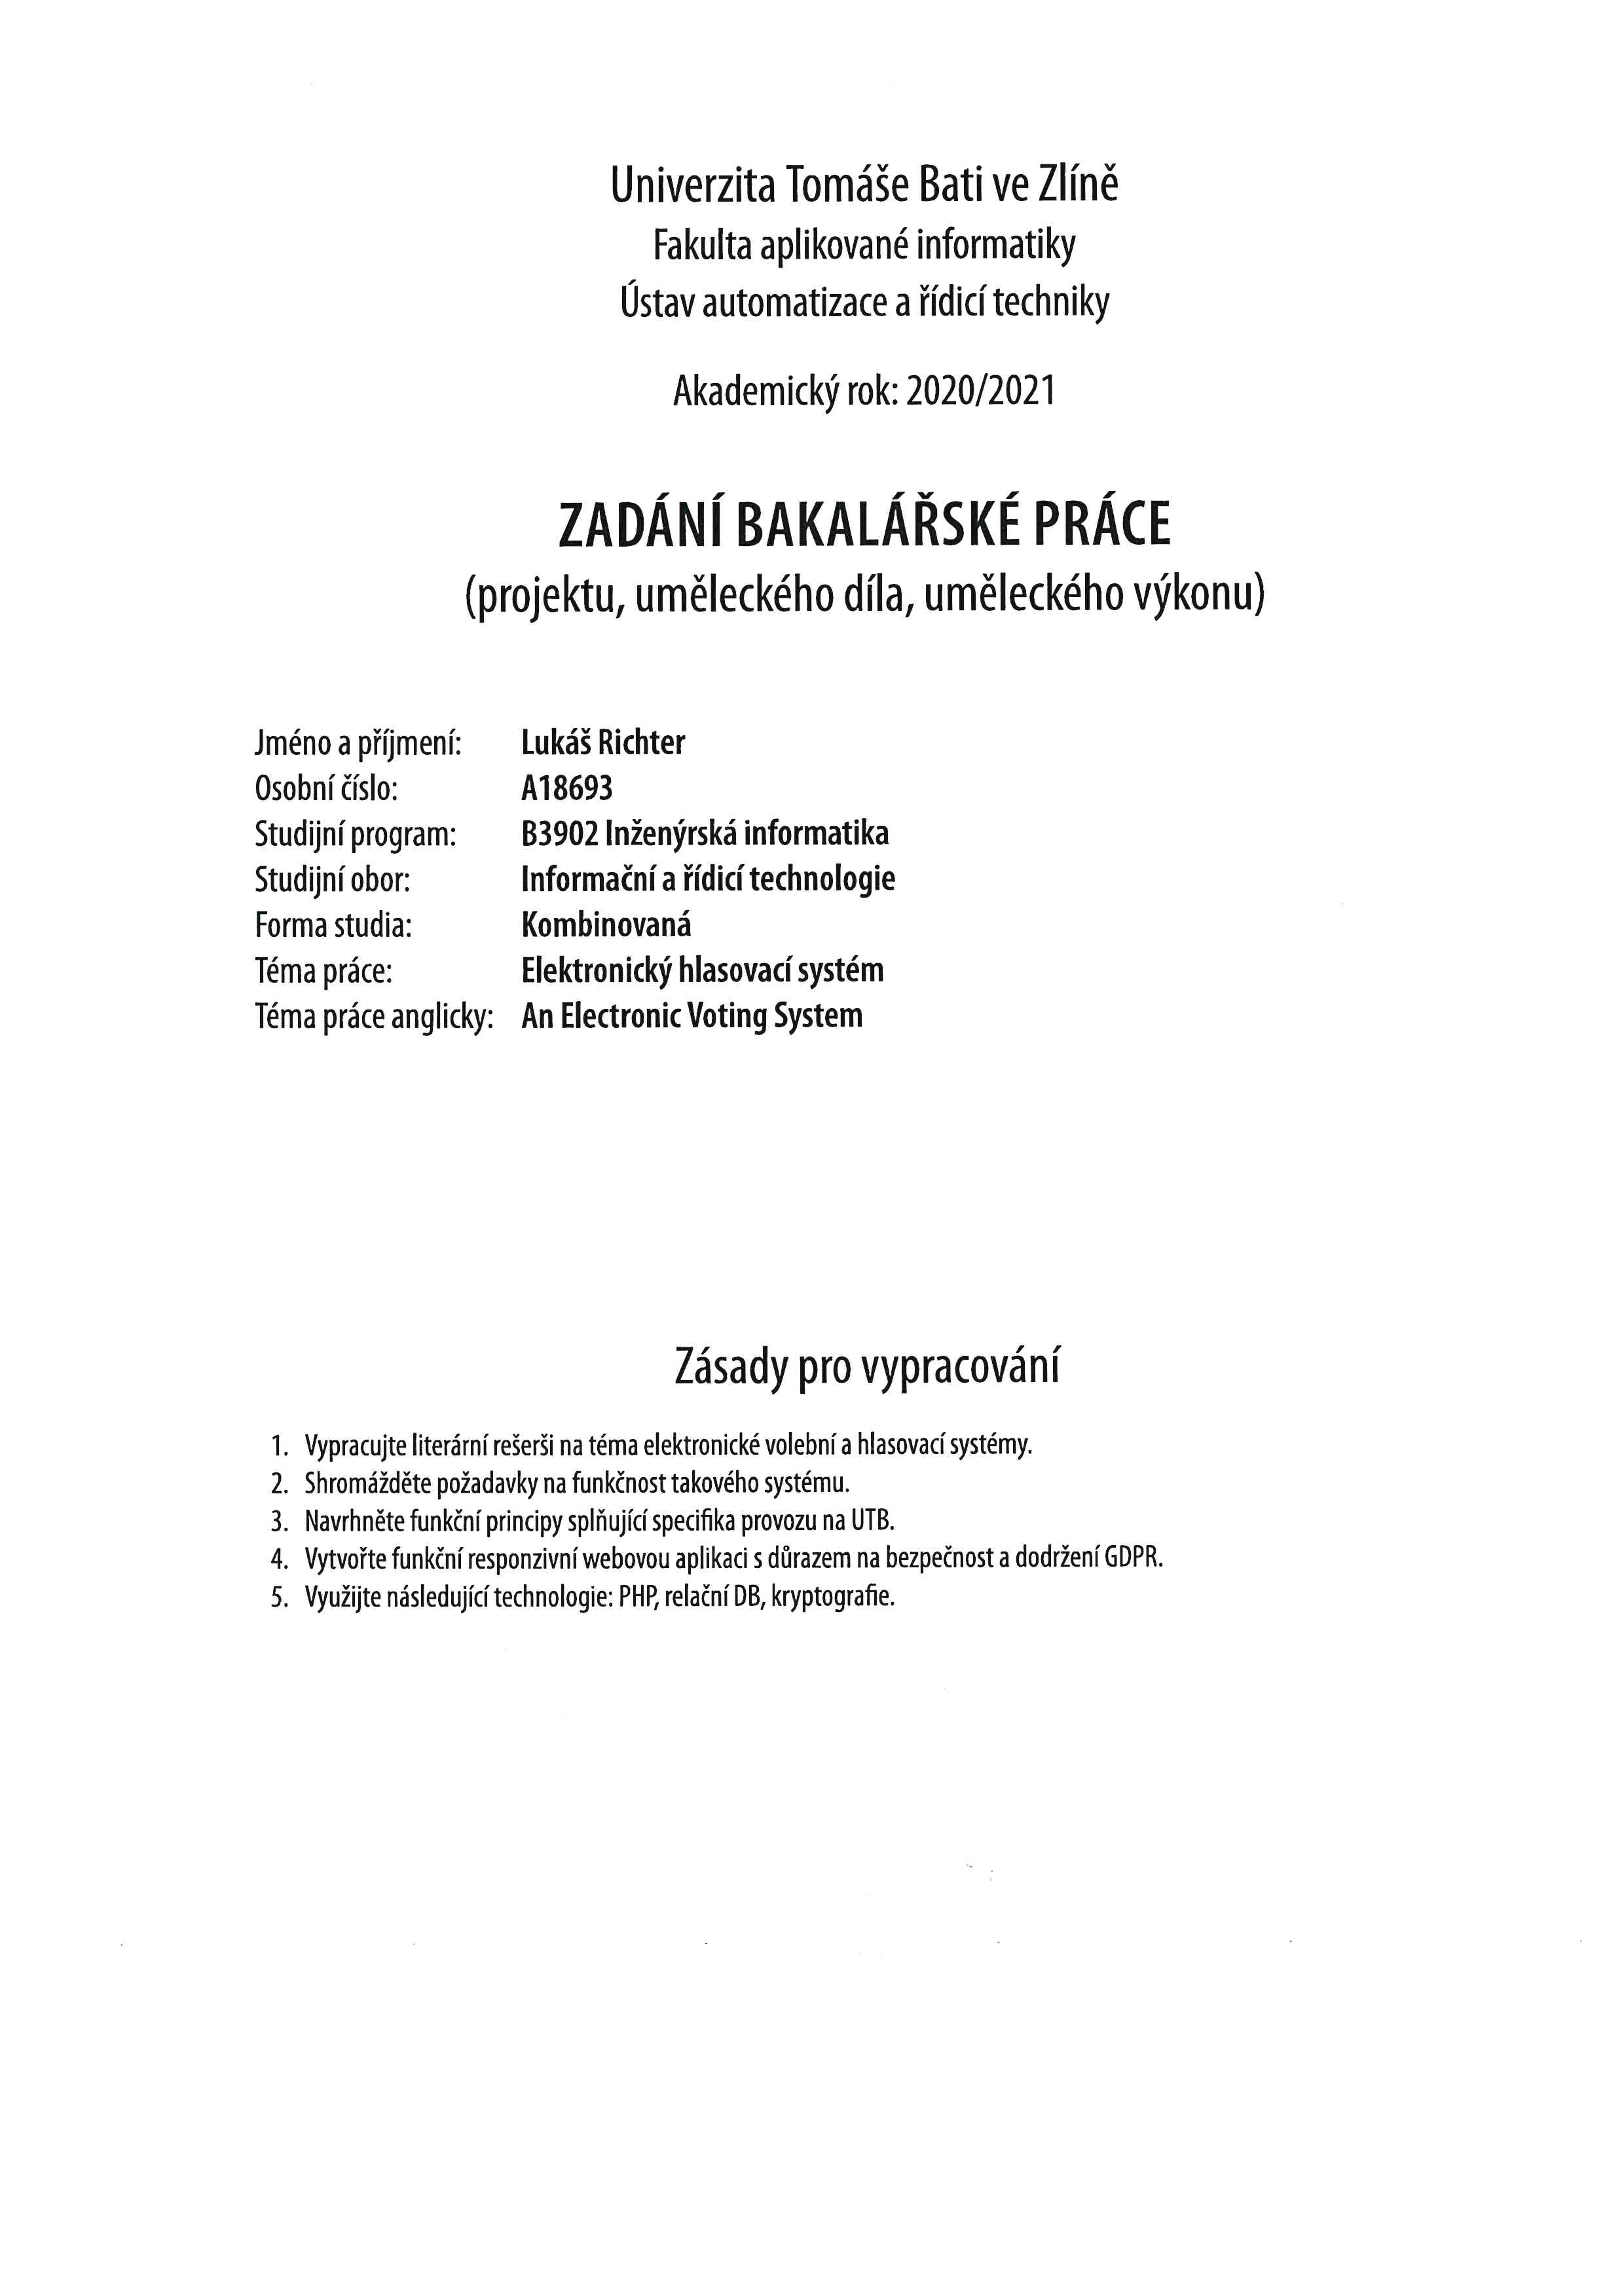
\includegraphics[height=\textheight]{graphics/zadani_A.png}}
\end{figure*}


\clearpage
\thispagestyle{empty}
\begin{figure*}[tp]
  \noindent\makebox[\textwidth]{%
	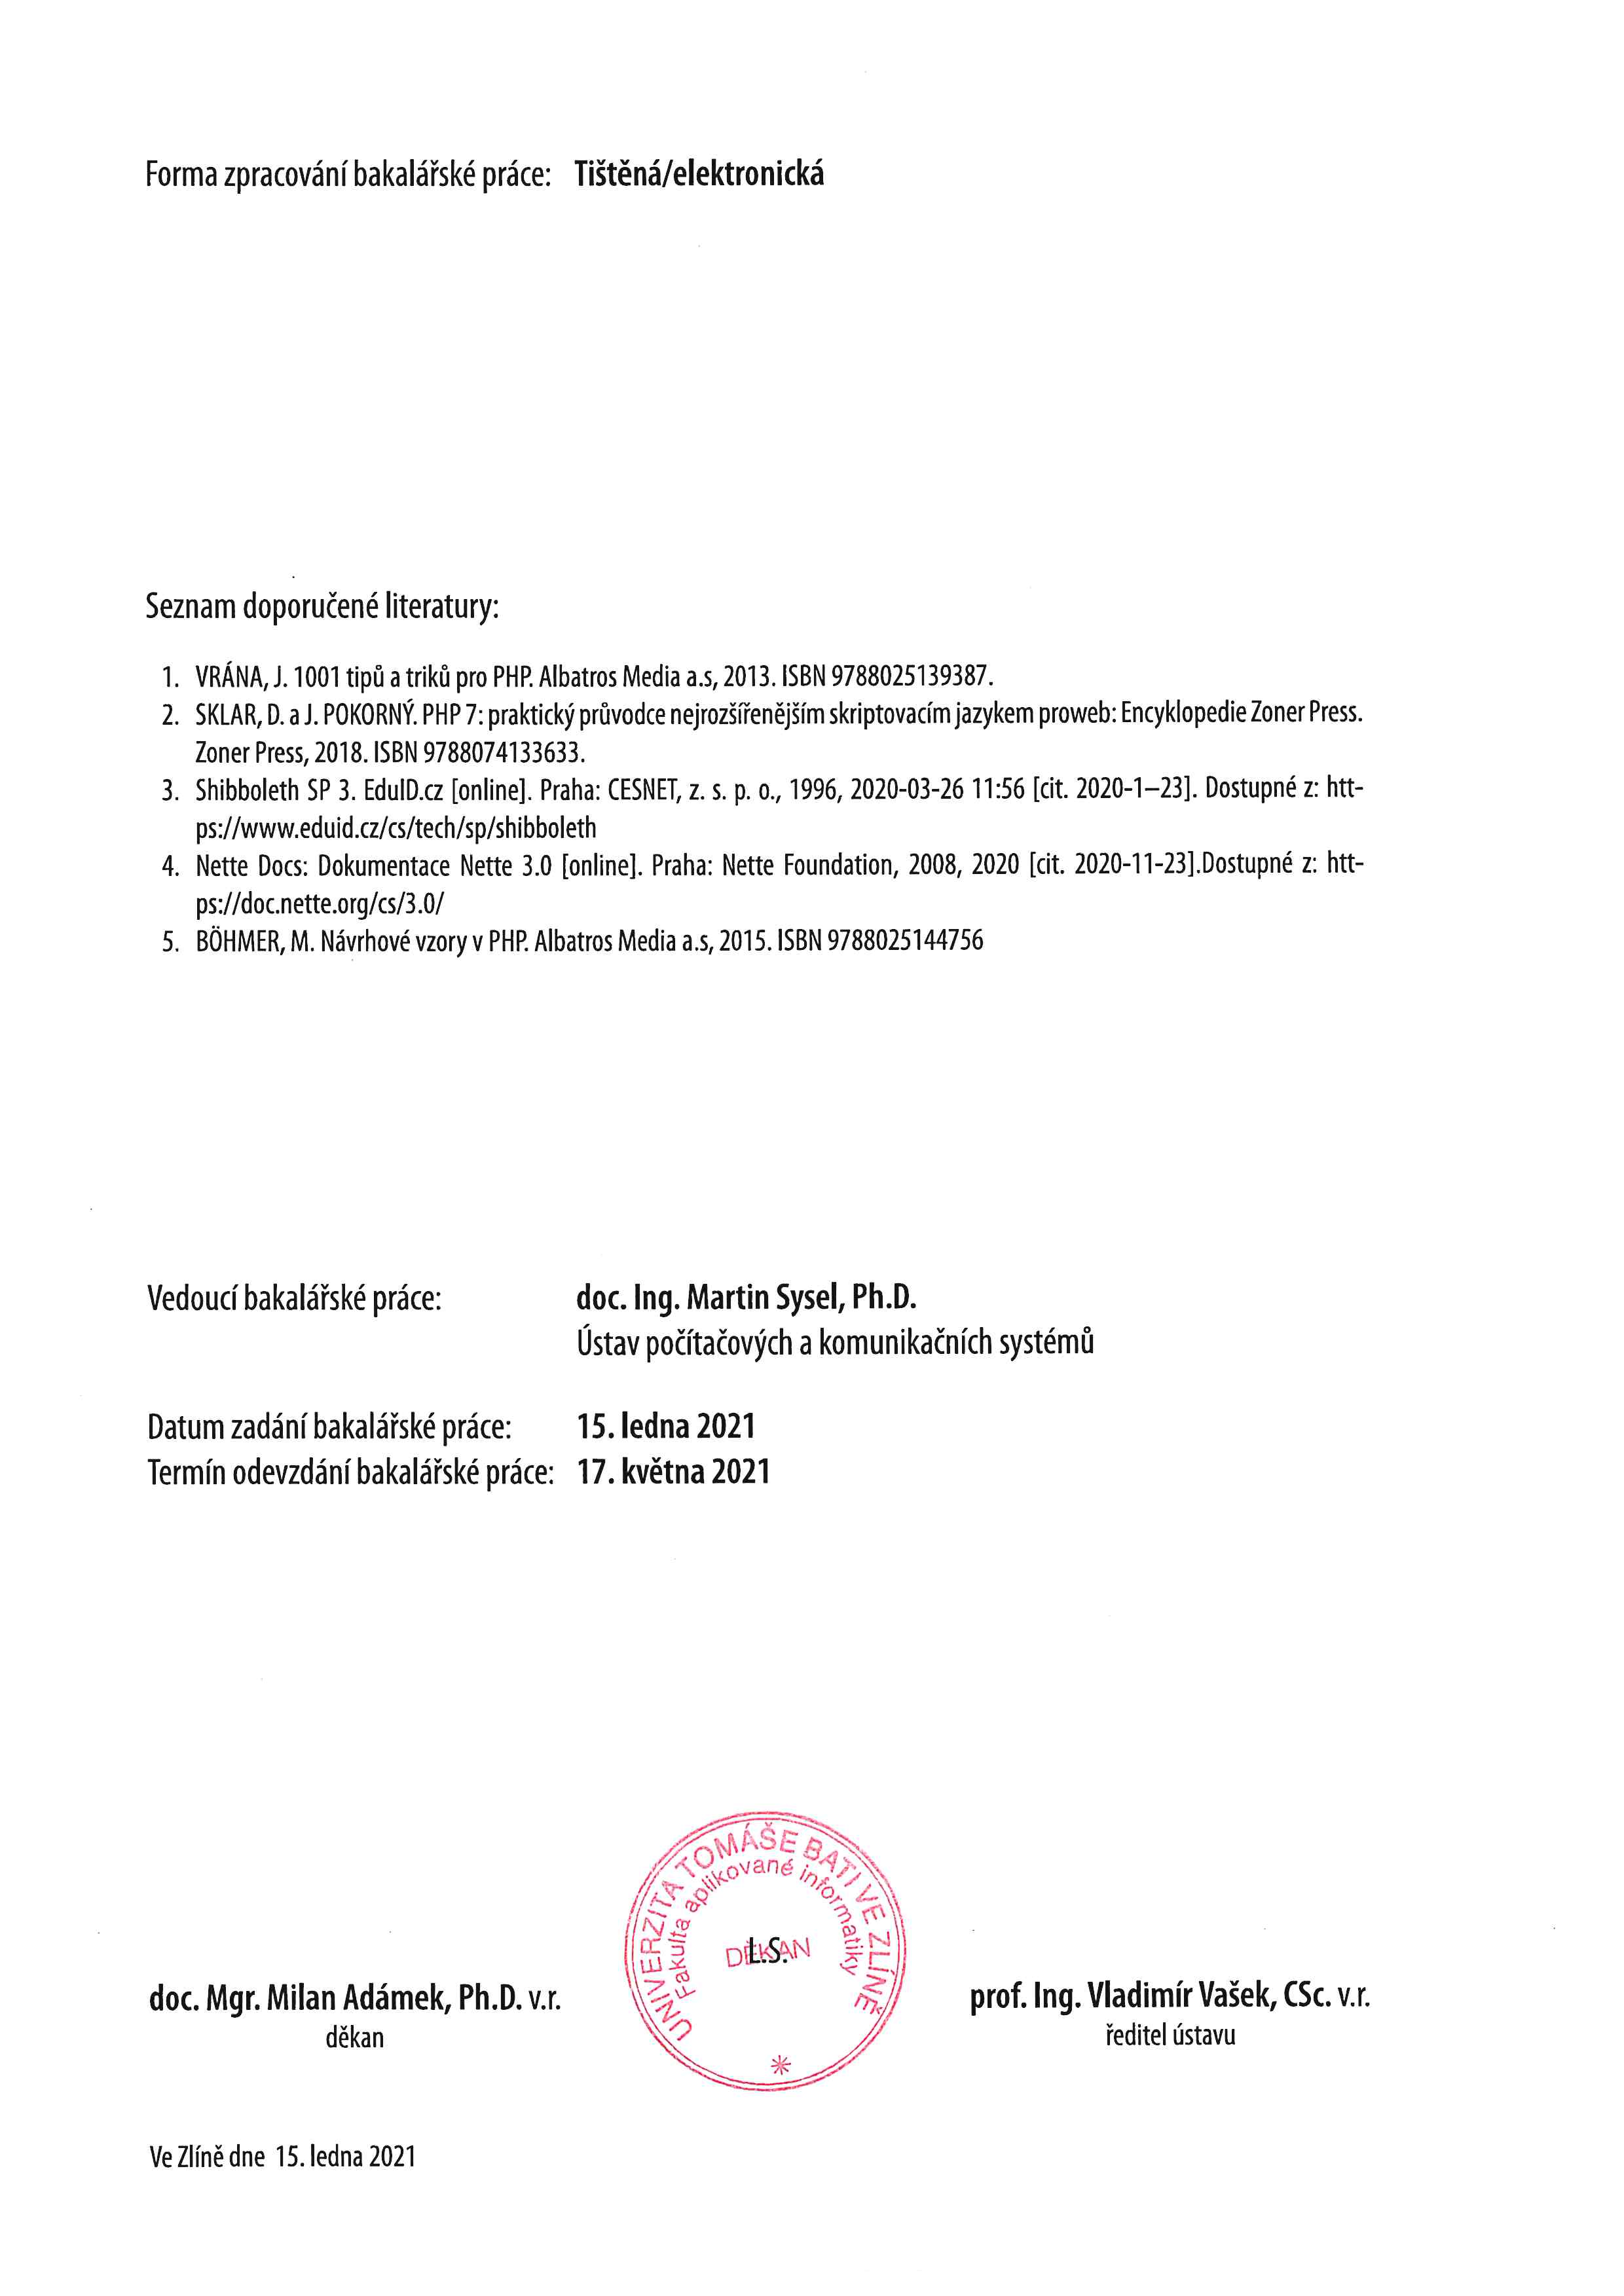
\includegraphics[height=\textheight]{graphics/zadani_B.png}}
\end{figure*}


}

% Nastaveni zobrazovani zahlavi dokumentu
\newcommand{\aktivujZahlavi}{
	\renewcommand{\headrulewidth}{1pt}
	\rhead{\thepage}
	
	\ifczech
		\lhead{\b{UTB ve Zlíně, \ifthenelse{\equal{\fakulta}{FAI}}{Fakulta aplikované informatiky}{\ifthenelse{\equal{\fakulta}{FAME}}{Fakulta managementu a ekonomiky}{\ifthenelse{\equal{\fakulta}{FHS}}{Fakulta humanitních studií}{\ifthenelse{\equal{\fakulta}{FLKR}}{Fakulta logistiky a krizového řízení}{\ifthenelse{\equal{\fakulta}{FMK}}{Fakulta multimediálních komunikací}{\ifthenelse{\equal{\fakulta}{FT}}{Fakulta technologická}{\ifthenelse{\equal{\fakulta}{UNI}}{Univerzitní institut}{}}}}}}}}}
	\else \ifenglish
		\lhead{\b{TBU in Zlín, \ifthenelse{\equal{\fakulta}{FAI}}{Faculty of Applied Informatics}{\ifthenelse{\equal{\fakulta}{FAME}}{Faculty of Management and Economics}{\ifthenelse{\equal{\fakulta}{FHS}}{Faculty of Humanities}{\ifthenelse{\equal{\fakulta}{FLKR}}{Faculty of Logistics and Crisis Management}{\ifthenelse{\equal{\fakulta}{FMK}}{Faculty of Multimedia Communications}{\ifthenelse{\equal{\fakulta}{FT}}{Faculty of Technology}{\ifthenelse{\equal{\fakulta}{UNI}}{University Institute}{}}}}}}}}}
	\fi \fi
}

% Příkaz \logopracerok vloží na dané místo logo fakulty, typ práce a rok
\newcommand{\logopracerok}{
	\ifczech
		\iffai  \put(82.2,-223.3){\makebox(84,16.4){
\includegraphics[width=90mm]{graphics/logo/fai_logo_cz.png}}} \fi
		\iffame \put(82.2,-223.3){\makebox(84,16.4){
\includegraphics[width=90mm]{graphics/logo/fame_logo_cz.png}}} \fi
		\iffhs  \put(82.2,-223.3){\makebox(84,16.4){
\includegraphics[width=90mm]{graphics/logo/fhs_logo_cz.png}}} \fi
		\ifflkr \put(82.2,-223.3){\makebox(84,16.4){
\includegraphics[width=90mm]{graphics/logo/flkr_logo_cz.png}}} \fi
		\iffmk  \put(82.2,-223.3){\makebox(84,16.4){
\includegraphics[width=90mm]{graphics/logo/fmk_logo_cz.png}}} \fi
		\ifft   \put(82.2,-223.3){\makebox(84,16.4){
\includegraphics[width=90mm]{graphics/logo/ft_logo_cz.png}}} \fi
		\ifuni  \put(82.2,-223.3){\makebox(84,16.4){
\includegraphics[width=90mm]{graphics/logo/uni_logo_cz.png}}} \fi
	\else \ifenglish
		\iffai  \put(82.2,-223.3){\makebox(84,16.4){
\includegraphics[width=90mm]{graphics/logo/fai_logo_en.png}}} \fi
		\iffame \put(82.2,-223.3){\makebox(84,16.4){
\includegraphics[width=90mm]{graphics/logo/fame_logo_en.png}}} \fi
		\iffhs  \put(82.2,-223.3){\makebox(84,16.4){
\includegraphics[width=90mm]{graphics/logo/fhs_logo_en.png}}} \fi
		\ifflkr \put(82.2,-223.3){\makebox(84,16.4){
\includegraphics[width=90mm]{graphics/logo/flkr_logo_en.png}}} \fi
		\iffmk  \put(82.2,-223.3){\makebox(84,16.4){
\includegraphics[width=90mm]{graphics/logo/fmk_logo_en.png}}} \fi
		\ifft   \put(82.2,-223.3){\makebox(84,16.4){
\includegraphics[width=90mm]{graphics/logo/ft_logo_en.png}}} \fi
		\ifuni  \put(82.2,-223.3){\makebox(84,16.4){
\includegraphics[width=90mm]{graphics/logo/uni_logo_en.png}}} \fi
	\fi \fi
	\put(0,-205){\linethickness{1pt}\line(1,0){170}}
	\ifczech
		\ifbp \put(4,-215){\makebox(69.5,4.5)[l]{\noindent\fontsize{16}{1}\usefont{OT1}{lmss}{m}{n}Bakalářská práce}} \fi
		\ifdp \put(4,-215){\makebox(69.5,4.5)[l]{\noindent\fontsize{16}{1}\usefont{OT1}{phv}{m}{n}Diplomová práce}} \fi
	\else \ifenglish
		\ifbp \put(4,-215){\makebox(69.5,4.5)[l]{\noindent\fontsize{16}{1}\usefont{OT1}{phv}{m}{n}Bachelor's thesis}} \fi
		\ifdp \put(4,-215){\makebox(69.5,4.5)[l]{\noindent\fontsize{16}{1}\usefont{OT1}{phv}{m}{n}Master's thesis}} \fi
	\fi \fi
	\put(4,-220){\makebox(69.5,4.5)[l]{\noindent\fontsize{16}{1}\usefont{OT1}{lmss}{m}{n}\rok}}
	\put(0,-225){\linethickness{1pt}\line(1,0){170}}
	\put(75,-223.3){\linethickness{1pt}\line(0,1){16.4}}
}

% Úvodní stránka s logem fakulty
\newcommand{\titulnistrana}{
	\thispagestyle{empty}
	\voffset=-2.01cm\evensidemargin=0pt\oddsidemargin=0cm\parindent=0pt\headsep=0pt\headheight=0pt\parskip=0pt\textheight=272mm\textwidth=200mm
	\renewcommand{\baselinestretch}{0}
	
	\setlength{\unitlength}{1mm}
	\begin{picture}(-10,8)
		\ifczech
			% Nazev prace
			%\put(0,-100){\makebox(170,50){\fontsize{24}{1}\usefont{OT1}{phv}{b}{n}#1}}
			%		\put(0,-100){\makebox(170,50){\protect\parbox{0.8\textwidth}{\protect\centering\fontsize{24}{1}\usefont{OT1}{phv}{b}{n}#1}}}
			
			% Vyreseno odradkovani
			\put(0,-100){\makebox(170,50){\protect\parbox{0.8\textwidth}{\protect\centering\setstretch{2.0}\usefont{OT1}{lmss}{b}{n}{\Huge\nazevcz}}}}
			
			% Jmeno autora
			\put(0,-135){\makebox(170,25){\fontsize{20}{1}\usefont{OT1}{lmss}{m}{n}\autor}}
		\else \ifenglish
			% Nazev prace
			%\put(0,-100){\makebox(170,50){\fontsize{24}{1}\usefont{OT1}{phv}{b}{n}#1}}
			%\put(0,-95){\makebox(170,50){\protect\parbox{0.8\textwidth}{\protect\centering\fontsize{24}{1}\usefont{OT1}{phv}{b}{n}#1}}}
			%\put(0,-88)%toto bylo pouzito v pripade zobrazeni nazvu ve dvou jazycich
			\put(0,-100){\makebox(170,50){\protect\parbox{0.8\textwidth}{\protect\centering\setstretch{2.0}\usefont{OT1}{lmss}{b}{n}{\Huge\nazeven}}}}
	
			%\put(0,-111){\makebox(170,50){\fontsize{20}{1}\usefont{OT1}{phv}{m}{n}#1}}
			%\put(0,-116){\makebox(170,50){\protect\parbox{0.8\textwidth}{\protect\centering\fontsize{20}{1}\usefont{OT1}{phv}{m}{n}#2}}}
			%\put(0,-115){\makebox(170,50){\protect\parbox{0.8\textwidth}{\protect\centering\setstretch{1.5}\usefont{OT1}{phv}{m}{n}{\Large\nazevcz}}}}
			
			% Jmeno autora
			\put(0,-135){\makebox(170,25){\fontsize{20}{1}\usefont{OT1}{lmss}{m}{n}\autor}}
		\fi \fi
		\logopracerok
	\end{picture}
}


% Strana s abstraktem a klíčovými slovy v češtině a angličtině
\newcommand{\abstraktaklicovaslova}{
	\clearpage
	\thispagestyle{empty}
	\nm{Abstrakt}
	\abstraktcz
	
	\vspace{1cm}
	Klíčová slova: \klicovaslovacz
	
	\vspace{3cm}
	
	\nns{Abstract}
	\abstrakten
	
	\vspace{1cm}
	Keywords: \klicovaslovaen
}


% ============================================================================ %
% NASTAVENÍ ZOBRAZENÍ PŘÍLOH -- SEZNAM, ČÍSLOVÁNÍ, VLASTNÍ STYL

\makeatletter % tímto příkazem dávám najevo, že budu editovat přímo příkazy ze šablony

% definice seznamu příloh - příkaz \listofappendices
\def\listofappendices{%
	\newpage
	\phantomsection
	\setcounter{section}{0}
	\ifczech
		\addcontentsline{toc}{section}{Seznam příloh}
		\@restonecolfalse\if@twocolumn\@restonecoltrue\onecolumn\fi
		\section*{SEZNAM PŘÍLOH}
	\else \ifenglish
		\addcontentsline{toc}{section}{List of Appendices}
		\@restonecolfalse\if@twocolumn\@restonecoltrue\onecolumn\fi
		\section*{LIST OF APPENDICES}
	\fi \fi
	\@mkboth{LIST OF APPENDICES}{LIST OF APPENDICES}
	\@starttoc{loa}\if@restonecol\twocolumn\fi
	\pagestyle{empty}
	\thispagestyle{fancy}
}

\def\ext@appendix{loa}
\def\tocname{loa}

% definice příkazu \priloha{nazev prilohy} pro vložení nové přílohy
\newcommand{\priloha}[1]{
	\clearpage
	\refstepcounter{section}
	%\voffset=-3cm  % vertikalni posun
	\addtocontents{loa}{\protect\makebox[1.5cm][l]{\ifczech P\else \ifenglish A\fi\fi\ \@Roman\c@section.} #1\newline}
	\ifczech
		{\bf PŘÍLOHA P \@Roman\c@section. \MakeTextUppercase{#1}}
	\else \ifenglish
		{\bf APPENDIX A \@Roman\c@section. \MakeTextUppercase{#1}}
	\fi	\fi
	\par
}

% ============================================================================ %
% OBSAH: NASTAVENÍ VELKÝCH PÍSMEN PRO NÁZVY SEKCÍ A HLAVNÍCH NADPISŮ

\let\oldcontentsline\contentsline
\def\contentsline#1#2{%
  \expandafter\ifx\csname l@#1\endcsname\l@section
    \expandafter\@firstoftwo
  \else
    \expandafter\@secondoftwo
  \fi
  {%
    \oldcontentsline{#1}{\MakeTextUppercase{#2}}%
  }{%
    \oldcontentsline{#1}{#2}%
  }%
}

\def\@part[#1]#2{
	\ifnum \c@secnumdepth >\m@ne
		\refstepcounter{part}
		\addcontentsline{toc}{section}{\protect\texorpdfstring{\makebox[0.85cm]{\thepart\hfill} #1}{\thepart\ #1}}
	\else
		\addcontentsline{toc}{section}{#1}
	\fi
	{\parindent \z@ \raggedright
	\interlinepenalty \@M
	\clearpage
	\normalfont
    \ifnum \c@secnumdepth >\m@ne
    	\Large\bfseries
		\nobreak
	\fi
	\vspace*{9cm}
	\center\huge \bfseries\thepart. \MakeTextUppercase{#2}
	\markboth{}{}\par}
	\nobreak
	\clearpage
    \@afterheading
}


% ============================================================================ %
% NASTAVENÍ FORMÁTU ČÍSLOVÁNÍ OBRÁZKŮ A TABULEK

\def\thefigure{\arabic{figure}}      % číslování obrázků typu (y)
\def\thetable{\arabic{table}}        % číslování tabulek typu (y)
\captiondelim{. } % změníme dvoutečku za Obr/Tab za tečku

% Nastavení číslování obrázků, tabulek i rovnic do formátu <číslo kapitoly>.<pořadové číslo>
\counterwithin{figure}{section}
\counterwithin{table}{section}
\counterwithin{equation}{section}

% Odsazeni popisku v seznamu obrazku a tabulek
\patchcmd{\@caption}{\csname the#1\endcsname}{\csname fnum@#1\endcsname}{}{}
%{\renewcommand*\numberline[1]{Fig. \,#1\space}}
%\renewcommand*\l@figure{\@dottedtocline{1}{0em}{5.0em}}
%\renewcommand*\l@table{\@dottedtocline{1}{0em}{5.0em}}

% Vynulování čítačů
\@addtoreset{table}{section}
\@addtoreset{figure}{section}
\@addtoreset{footnote}{section}
	
\makeatother % a to je ukončení \makeatletter


% ============================================================================ %
% ÚPRAVA VZHLEDU OBSAHU, SEZNAMU OBRÁZKŮ A TABULEK

% nastavení vertikální mezery před stylem část, nadpis 1--3
\setlength{\cftbeforepartskip}{3pt}
\setlength{\cftbeforesecskip}{3pt}
\setlength{\cftbeforesubsecskip}{3pt}
\setlength{\cftbeforesubsubsecskip}{0cm}

% odsazení zleva pro styl část, nadpis 1--3
\setlength{\cftpartindent}{0cm}
\setlength{\cftsecindent}{0cm}
\setlength{\cftsubsecindent}{0cm}
\setlength{\cftsubsubsecindent}{0cm}

% nastavení fontu pro styl část, nadpis 1--3
\renewcommand{\cftpartfont}{\small\bfseries}
\renewcommand{\cftsecfont}{\small\bfseries}
\renewcommand{\cftsubsecfont}{\scshape}
\renewcommand{\cftsubsubsecfont}{}

% odsazení čísla a textu titulku pro styl část, nadpis 1--3
\cftsetindents{part}{0cm}{1cm}
\cftsetindents{sec}{0cm}{1cm}
\cftsetindents{subsec}{0.5cm}{1.25cm}
\cftsetindents{subsubsec}{1cm}{1.5cm}
\cftsetindents{fig}{0cm}{1.5cm}
\cftsetindents{tab}{0cm}{1.5cm}

% nastavení vodící čáry pro styl část, nadpis 1--3, obrázky a tabulky
\renewcommand{\cftdot}{\ensuremath{.}} % tímto příkazem lze změnit vodící tečky v obsahu na jiný znak
\renewcommand{\cftpartleader}{\cftdotfill{0.3}}
\renewcommand{\cftsecleader}{\cftdotfill{0.3}}
\renewcommand{\cftsubsecleader}{\cftdotfill{0.3}}
\renewcommand{\cftsubsubsecleader}{\cftdotfill{0.3}}
\renewcommand{\cftfigleader}{\cftdotfill{0.3}}
\renewcommand{\cfttableader}{\cftdotfill{0.3}}

% změna fontu pro text "Obsah", "Seznam obrázků" a "Seznam tabulek"
\renewcommand{\cfttoctitlefont}{\normalsize\bfseries\thispagestyle{empty}}
\renewcommand{\cftloftitlefont}{\normalsize\bfseries\thispagestyle{fancy}}
\renewcommand{\cftlottitlefont}{\normalsize\bfseries\thispagestyle{fancy}}

\renewcommand{\cfttabpresnum}{Tab. }
\renewcommand{\cftfigaftersnum}{.}
\renewcommand{\cfttabaftersnum}{.}
\setlength{\cftfignumwidth}{5em}
\setlength{\cfttabnumwidth}{5em}


% ============================================================================ %
% NASTAVENÍ FONTU PRO NADPISY

\sectionfont{\normalsize}
\subsectionfont{\normalsize\bfseries}
\subsubsectionfont{\small\bfseries}
\paragraphfont{\small\bf}

% definice nového stylu \comment -- komentář k šabloně
\newcommand{\koment}[1]{\color{red}[#1]\color{black}}


% ============================================================================ %
% VSTUPY

% Nastaveni a kontrola fakulty
\newcommand{\nastavfakultu}[1]{
	\newcommand{\fakulta}{#1}
	\newif\iffai  \let\iffai\iffalse
	\newif\iffame \let\iffame\iffalse
	\newif\iffhs  \let\iffhs\iffalse
	\newif\ifflkr \let\ifflkr\iffalse
	\newif\iffmk  \let\iffmk\iffalse
	\newif\ifft   \let\ifft\iffalse
	\newif\ifuni  \let\ifuni\iffalse
	
	\ifthenelse{\equal{#1}{FAI}}{\let\iffai\iftrue}{}
	\ifthenelse{\equal{#1}{FAME}}{\let\iffame\iftrue}{}
	\ifthenelse{\equal{#1}{FHS}}{\let\iffhs\iftrue}{}
	\ifthenelse{\equal{#1}{FLKR}}{\let\ifflkr\iftrue}{}
	\ifthenelse{\equal{#1}{FMK}}{\let\iffmk\iftrue}{}
	\ifthenelse{\equal{#1}{FT}}{\let\ifft\iftrue}{}
	\ifthenelse{\equal{#1}{UNI}}{\let\ifuni\iftrue}{}
	
	\iffai \else \iffame \else \iffhs \else \ifflkr \else \iffmk \else \ifft \else \ifuni \else
		\errmessage{Chyba nastaveni fakulty}
	\fi \fi \fi \fi \fi \fi \fi
}

% Nastaveni a kontrola typu prace
\newcommand{\nastavtyp}[1]{
	\newcommand{\typ}{#1}
	
	\newif\ifbp \let\ifbp\iffalse
	\newif\ifdp \let\ifdp\iffalse
	
	\ifthenelse{\equal{#1}{BP}}{\let\ifbp\iftrue}{}
	\ifthenelse{\equal{#1}{DP}}{\let\ifdp\iftrue}{}
	
	\ifbp \else \ifdp \else
		\errmessage{Chyba nastaveni typu prace}
	\fi \fi
}

% Nastaveni roku
\newcommand{\nastavrok}[1]{
	\newcommand{\rok}{#1}
}

% Nastaveni jmena
\newcommand{\nastavautora}[1]{
	\newcommand{\autor}{#1}
}

% Nastaveni nazvu
\newcommand{\nastavnazevcz}[1]{
	\newcommand{\nazevcz}{#1}
}
\newcommand{\nastavnazeven}[1]{
	\newcommand{\nazeven}{#1}
}

% Nastaveni abstraktu
\newcommand{\nastavabstraktcz}[1]{
	\newcommand{\abstraktcz}{#1}
}
\newcommand{\nastavabstrakten}[1]{
	\newcommand{\abstrakten}{#1}
}

% Nastaveni klicovych slov
\newcommand{\nastavklicovaslovacz}[1]{
	\newcommand{\klicovaslovacz}{#1}
}
\newcommand{\nastavklicovaslovaen}[1]{
	\newcommand{\klicovaslovaen}{#1}
}

% Nastaveni a kontrola jazyka
\newcommand{\nastavjazyk}[1]{
	\newcommand{\jazyk}{#1}
	
	\newif\ifczech   \let\ifczech\iffalse
	\newif\ifenglish \let\ifenglish\iffalse
	
	\ifthenelse{\equal{#1}{CZ}}{\let\ifczech\iftrue}{}
	\ifthenelse{\equal{#1}{EN}}{\let\ifenglish\iftrue}{}
	
	\ifczech \else \ifenglish \else
		\errmessage{Chyba nastaveni jazyka}
	\fi \fi
	
	\ifczech
		\usepackage[czech]{babel}
		% Vlastni definice nazvu
		\addto\captionsczech{\renewcommand{\contentsname}{\MakeTextUppercase{Obsah}}}
		\addto\captionsczech{\renewcommand{\refname}{\MakeTextUppercase{Seznam použité literatury}}}
		\addto\captionsczech{\renewcommand{\listfigurename}{\MakeTextUppercase{Seznam obrázků}}}
		\addto\captionsczech{\renewcommand{\listtablename}{\MakeTextUppercase{Seznam tabulek}}}
		%\addto\captionsczech{\renewcommand{\figurename}{Obr.}}
		%\addto\captionsczech{\renewcommand{\tablename}{Tab.}}
		\renewcommand{\cftfigpresnum}{Obr. }
	\else \ifenglish
		\usepackage[english]{babel}	
		% Vlastni definice nazvu
		\addto\captionsenglish{\renewcommand{\contentsname}{\MakeTextUppercase{Table of Contents}}}
		\addto\captionsenglish{\renewcommand{\refname}{\MakeTextUppercase{References}}}
		\addto\captionsenglish{\renewcommand{\listfigurename}{\MakeTextUppercase{List of Figures}}}
		\addto\captionsenglish{\renewcommand{\listtablename}{\MakeTextUppercase{List of Tables}}}
		%\addto\captionsenglish{\renewcommand{\figurename}{Fig.}}
		%\addto\captionsenglish{\renewcommand{\tablename}{Tab.}}
		\renewcommand{\cftfigpresnum}{Fig. }
	\fi \fi
}


% Nastaveni vertikalniho odsazeni nad rovnicemi/soustavami rovnic (prvni parametr),
% a pod (druhy parametr)
\newcommand{\nastavmezerukolemrovnic}[2]{
	\let\oldequation=\equation
	\let\endoldequation=\endequation
	\renewenvironment{equation}{\vspace{#1}\begin{oldequation}}{\end{oldequation}\vspace{#2}}
	
	\let\oldeqnarray=\eqnarray
	\let\endoldeqnarray=\endeqnarray
	\renewenvironment{eqnarray}{\vspace{#1}\begin{oldeqnarray}}{\end{oldeqnarray}\vspace{#2}}
}

% Nastaveni vertikalniho odsazeni nad tabulkami (prvni parametr),
% a pod (druhy parametr)
\newcommand{\nastavmezerukolemtabulek}[2]{
	\let\oldtable=\table
	\let\endoldtable=\endtable
	\renewenvironment{table}{\vspace{#1}\begin{oldtable}}{\end{oldtable}\vspace{#2}}
}

% Nastaveni vertikalniho odsazeni nad obrazky (prvni parametr),
% a pod (druhy parametr)
\newcommand{\nastavmezerukolemobrazku}[2]{
	\let\oldfigure=\figure
	\let\endoldfigure=\endfigure
	\renewenvironment{figure}{\vspace{#1}\begin{oldfigure}}{\end{oldfigure}\vspace{#2}}
}


% ============================================================================ %
% STRANA S PROHLASENIM

\newcommand{\prohlaseni}{{
	\clearpage
	\thispagestyle{empty}

	\ifczech
	\textbf{Prohlašuji, že}
	\begin{itemize}
		\setlength{\parskip}{0pt}
		\setlength{\itemsep}{0pt}
		\setstretch{1.05}
		\item{beru na vědomí, že odevzdáním \ifbp bakalářské \else \ifdp diplomové \fi \fi práce souhlasím se zveřejněním své práce podle zákona č. 111/1998 Sb. o vysokých školách a o změně a doplnění dalších zákonů (zákon o vysokých školách), ve znění pozdějších právních předpisů, bez ohledu na výsledek obhajoby;}
		\item{beru na vědomí, že \ifbp bakalářské \else \ifdp diplomové \fi \fi práce bude uložena v~elektronické podobě v univerzitním informačním systému dostupná k prezenčnímu nahlédnutí, že jeden výtisk \ifbp bakalářské \else \ifdp diplomové \fi \fi práce bude uložen v příruční knihovně \iffai Fakulty aplikované informatiky. \else \iffame Fakulty managementu a ekonomiky. \else \iffhs Fakulty humanitních studií. \else \ifflkr Fakulty logistiky a krizového řízení. \else \iffmk Fakutly mutimediálních komunikací. \else \ifft Fakulty technologické. \else \ifuni Univerzitního institutu. \if \fi \fi \fi \fi \fi \fi \fi \fi Univerzity Tomáše Bati ve Zlíně; }
		\item{byl/a jsem seznámen/a s tím, že na moji \ifbp bakalářskou \else \ifdp diplomovou \fi \fi práci se plně vztahuje zákon č. 121/2000 Sb. o právu autorském, o právech souvisejících s právem autorským a o změně některých zákonů (autorský zákon) ve znění pozdějších právních předpisů, zejm. § 35 odst. 3;}
		\item{beru na vědomí, že podle § 60 odst. 1 autorského zákona má Univerzita Tomáše Bati ve Zlíně právo na uzavření licenční smlouvy o užití školního díla v rozsahu § 12 odst. 4 autorského zákona;}
		\item{beru na vědomí, že podle § 60 odst. 2 a 3 autorského zákona mohu užít své dílo –\ \ifbp bakalářskou \else \ifdp diplomovou \fi \fi práci nebo poskytnout licenci k~jejímu využití jen připouští-li tak licenční smlouva uzavřená mezi mnou a Univerzitou Tomáše Bati ve Zlíně s~tím, že vyrovnání případného přiměřeného příspěvku na úhradu nákladů, které byly Univerzitou Tomáše Bati ve Zlíně na vytvoření díla vynaloženy (až do jejich skutečné výše) bude rovněž předmětem této licenční smlouvy;}
		\item{beru na vědomí, že pokud bylo k vypracování \ifbp bakalářské \else \ifdp diplomové \fi \fi práce využito softwaru poskytnutého Univerzitou Tomáše Bati ve Zlíně nebo jinými subjekty pouze ke~studijním a výzkumným účelům (tedy pouze k~nekomerčnímu využití), nelze výsledky \ifbp bakalářské \else \ifdp diplomové \fi \fi práce využít ke komerčním účelům;}
		\item{beru na vědomí, že pokud je výstupem \ifbp bakalářské \else \ifdp diplomové \fi \fi práce jakýkoliv softwarový produkt, považují se za součást práce rovněž i zdrojové kódy, popř. soubory, ze~kterých se projekt skládá. Neodevzdání této součásti může být důvodem k~neobhájení práce.}
	\end{itemize}
	\medskip
	%\clearpage
	%\thispagestyle{empty}
	\textbf{Prohlašuji,}
	\begin{itemize}
		\setlength{\parskip}{0pt}
		\setlength{\itemsep}{0pt}
		\setstretch{1.05}
		\item{že jsem na \ifbp bakalářské \else \ifdp diplomové \fi \fi práci pracoval samostatně a použitou literaturu jsem citoval. V případě publikace výsledků budu uveden jako spoluautor.}
		\item{že odevzdaná verze \ifbp bakalářské \else \ifdp diplomové \fi \fi práce a verze elektronická nahraná do IS/STAG jsou totožné.}
	\end{itemize}
	\medskip
	Ve Zlíně, dne 14. května 2021 \hspace{6.5cm}
	
	\hspace{10.3cm}\textbf{Lukáš Richter} v.r.
	
	\else \ifenglish
	%\nm{THESIS AUTHOR STATEMENT}
	\textbf{I hereby declare that:}
	\begin{itemize}
		\setlength{\parskip}{0pt}
		\setlength{\itemsep}{0pt}
		\setstretch{1.05}
		\item{I understand that by submitting my \ifbp Bachelor's \else\ifdp Master's \fi\fi thesis, I agree to the publication of my work according to Law No. 111/1998, Coll., On Universities and on changes and amendments to other acts (e.g. the Universities Act), as amended by subsequent legislation, without regard to the results of the defence of the thesis.}		
		\item{I understand that my \ifbp Bachelor's \else\ifdp Master's \fi\fi Thesis will be stored electronically in the university information system and be made available for on-site inspection, and that a copy of the \ifbp Bachelor's \else\ifdp Master's \fi\fi Thesis will be stored in the Reference Library of the 
		\iffai Faculty of Applied Informatics, \else\iffame Faculty of Management and Economics, \else \iffhs Faculty of Humanities, \else\ifflkr Faculty of Logistics and Crisis Management, \else\iffmk Faculty of Multimedia Communications, \else\ifft Faculty of Technology, \else\ifuni University Institute, \if \fi \fi \fi \fi \fi \fi \fi \fi Tomas Bata University in Zlín.}
		\item{I am aware of the fact that my \ifbp Bachelor's \else\ifdp Master's \fi\fi Thesis is fully covered by Act No. 121/2000 Coll. On Copyright, and Rights Related to Copyright, as amended by some other laws (e.g. the Copyright Act), as amended by subsequent legislation; and especially, by §35, Para. 3.}
		\item{I understand that, according to §60, Para. 1 of the Copyright Act, Tomas Bata University in Zlín has the right to conclude licensing agreements relating to the use of scholastic work within the full extent of §12, Para. 4, of the Copyright Act.}
		\item{I understand that, according to §60, Para. 2, and Para. 3, of the Copyright Act, I may use my work – \ifbp Bachelor's \else\ifdp Master's \fi\fi Thesis, or grant a license for its use, only if permitted by the licensing agreement concluded between myself and Tomas Bata University in Zlín with a view to the fact that Tomas Bata University in Zlín must be compensated for any reasonable contribution to covering such expenses/costs as invested by them in the creation of the thesis (up until the full actual amount) shall also be a subject of this licensing agreement.}
		\item{I understand that, should the elaboration of the \ifbp Bachelor's \else\ifdp Master's \fi\fi Thesis include the use of software provided by Tomas Bata University in Zlín or other such entities strictly for study and research purposes (i.e. only for non-commercial use), the results of my \ifbp Bachelor's \else\ifdp Master's \fi\fi Thesis cannot be used for commercial purposes.}
		\item{I understand that, if the output of my \ifbp Bachelor's \else\ifdp Master's \fi\fi Thesis is any software product(s), this/these shall equally be considered as part of the thesis, as well as any source codes, or files from which the project is composed. Not submitting any part of this/these component(s) may be a reason for the non-defence of my thesis.}
	\end{itemize}
	\medskip
	%\clearpage
	%\thispagestyle{empty}
	\textbf{I herewith declare that:}
	\begin{itemize}
		\setlength{\parskip}{0pt}
		\setlength{\itemsep}{0pt}
		\setstretch{1.05}
		\item{I have worked on my thesis alone and duly cited any literature I have used. In the case of the publication of the results of my thesis, I shall be listed as co-author.}
		\item{The submitted version of the thesis and its electronic version uploaded to IS/STAG are both identical.}
	\end{itemize}
	\medskip
	In Zlín; dated: \hspace{6.5cm}\dots\dots\dots\dots\dots\dots\dots\dots\dots\dots

	\hspace{10.3cm}Student's Signature
	
	\fi \fi
}}

% ============================================================================ %

\usepackage{lmodern}
%\usepackage{inconsolata}
%\renewcommand{\ttdefault}{lmtt}
%\usepackage{times}
\usepackage{blindtext}
\usepackage{dirtree}
\usepackage[section]{minted}
\usepackage{fancyvrb}
\VerbatimFootnotes
\usemintedstyle{default}
\renewcommand\listingscaption{Fragment zdrojového kódu}
\renewcommand{\listoflistingscaption}{SEZNAM FRAGMENTŮ ZDROJOVÉHO KÓDU}

\usepackage{calc}

%\usepackage[none]{hyphenat}

\tolerance=1
\emergencystretch=\maxdimen
\hyphenpenalty=10000
\hbadness=10000

\graphicspath{{svg/}}

\definecolor{bgLight}{rgb}{0.95,0.95,0.95}

\newmintedfile{php}{
%startinline,
xleftmargin=20pt,
linenos,
fontsize=\footnotesize,
%fontseries=l,
frame=lines,
framesep=2mm,
tabsize=2,
breaklines=true,
}

\newmintedfile[phpsnippet]{php}{
startinline,
xleftmargin=20pt,
linenos,
fontsize=\footnotesize,
%fontseries=l,
frame=lines,
framesep=2mm,
tabsize=2,
breaklines=true,
}

\newminted{php}{
startinline,
xleftmargin=20pt,
linenos,
fontsize=\footnotesize,
%fontseries=l,
frame=lines,
framesep=2mm,
tabsize=2,
breaklines=true,
}

\newmintinline{php}{
%startinline,
%bgcolor=bgLight,
fontseries=m,
%breaklines=true,
%breakanywhere=true,
}

\def\seznamkodu{
	\clearpage
	\phantomsection
	\listoflistings
	\clearpage
}

\def\svgobr#1#2#3#4{
	\begin{figure}[h]
		\centering \small \fontfamily{lmtt}\fontseries{l}\selectfont
%		\def\svgscale{#3}
		\def\svgwidth{#3\columnwidth}
		\input{svg/#4.pdf_tex}
		\normalsize \sffamily
		\captionsetup{width=\linewidth}
		\caption{#1}
		\label{#2}
		
	\end{figure}
}

\def\tt#1{
	\texttt{#1}
}

% Uživatelské definice -- upravte dle požadavků
\nastavfakultu{FAI}
	% FAI  -- pro Fakultu aplikované informatiky
	% FAME -- pro Fakultu managementu a ekonomiky
	% FHS  -- pro Fakultu humanitních studií
	% FLKR -- pro Fakultu logistiky a krizového řízení
	% FMK  -- pro Fakutlu mutimediálních komunikací
	% FT   -- pro Fakultu technologickou
	% UNI  -- pro Univerzitní institut
\nastavtyp{BP}
	% BP   -- bakalářská práce
	% DP   -- diplomová práce
\nastavrok{2021}
	% zadejte rok místo "xxxx"
\nastavjazyk{CZ}
	% CZ   -- práce bude v českém jazyce
	% EN   -- práce bude v anglickém jazyce

% Lze přidat vertikalni odsazeni nad (prvni parametr) a pod (druhy parametr)
% obrázky, tabulky i rovnice/soustavy rovnic
\nastavmezerukolemobrazku{0mm}{0mm}
\nastavmezerukolemtabulek{0mm}{0mm}
\nastavmezerukolemrovnic{0mm}{0mm}

\nastavautora{Lukáš Richter}
\nastavnazevcz{Elektronický hlasovací systém}
\nastavnazeven{Název práce anglicky (max. 2 řádky)} % Jen u anglicky psané práce
\nastavabstraktcz{Cílem této práce je návrh a implementace funkční volební a hlasovací aplikace. Primárním využitím jsou volby do akademických senátů na Univerzitě Tomáše Bati ve~Zlíně a hlasování na zasedáních akademických orgánů. Výsledný systém zaručuje dodržení principů elektronických voleb a poskytuje jednoduchý způsob, jak maximálně zpřístupnit volby co největšímu počtu uživatelů.

Aplikace je postavena na PHP frameworku Nette. Návrh aplikace umožňuje její relativně snadné modifikace co do rozmístění mezi několik serverů i nezávislost na~použitém systému řízení báze dat. Systém je navržen jako modulární a je možno ho dále rozšiřovat, např. o volitelné způsoby autentizace uživatelů.

Při návrhu bylo využito principu slepých digitálních podpisů a přímé komunikace klienta a serveru jako efektivního způsobu zajištění anonymity.}
\nastavabstrakten{The goal of this thesis is to design and implement functional electronic voting application. Primary use will be elections to Academic Senates of Tomas Bata University in Zlin  and voting of Academic Bodies.. The resulting system guarantees adherence to electronic voting principles and offers a simple solution how to make voting available to as many users as possible.

Application is based on PHP framework Nette. The design of the application allows its relatively simple modification in regards of distribution among multiple servers and independence on database management system used. System is designed as modular and it is possible to further extend it, e.g. with different user authentication options.

Blind digital signatures and direct client-server communication as an effective means to assure anonymity were used to desing the application.}
\nastavklicovaslovacz{Elektronické volby, e-voting, RSA, slepé podepisování, PHP, Domain Driven Design, MVC, Nette, Bootstrap}
\nastavklicovaslovaen{Electronic voting system, e-voting, RSA, Bling Signature, PHP, Domain Driven Design, MVC, Nette, Bootstrap}

% Následující příkaz nastaví standard PDF/A-1b
\aplikujpdfa


% ============================================================================ %
\begin{document}

\titulnistrana

\zadani

\prohlaseni

\abstraktaklicovaslova


% ============================================================================ %
\clearpage
\thispagestyle{empty}
Rád bych poděkoval doc. Ing. Martinu Syslovi, Ph.D. za cenné rady, věcné připomínky a vstřícnost při konzultacích během bakalářské práce.

\bigskip

\bigskip

\bigskip

Výzva představená zadáním práce mě zaujala možností vytvořit aplikaci od návrhu až po její finální implementaci. Aplikace zároveň není pouze teoretickým příkladem, ale~řešením reálného problému, které by mohlo být uplatněno v praxi. Vzhledem k~osobním zkušenostem s programováním webových aplikací věřím, že nabyté zkušenosti především z oboru kryptografie využiji i v profesním životě.

% ============================================================================ %
\obsah  % Obsah je generován automaticky


% ============================================================================ %
\OdsazovaniOdstavcuStart % Nastaví odsazování odstavců dle zvoleného jazyka

% ============================================================================ %
% Encoding: UTF-8 (žluťoučký kůň úpěl ďábelšké ódy)
% ============================================================================ %

% ============================================================================ %
\nn{Úvod}
První řádek prvního odstavce v kapitole či podkapitole se neodsazuje, ostatní ano. Vertikální odsazení mezy odstavci je typycké pro anglickou sazbu; czech babel toto respektuje, netřeba do textu přidávat jakékoliv explicitní formátování, viz ukázka sazby tohoto textu s následujícím odstavcem).

Formátování druhého odstavce. Text text text text text text text text text text text text.


% ============================================================================ %
\cast{Teoretická část}

\n{1}{Elektronické volby}
Na této stránce je k vidění způsob tvorby různých úrovní nadpisů.

\n{2}{Koncepce, výhody, nevýhody}
Text

\n{2}{Poždadvky, podmínky}
Text

\n{2}{RSA Blind Signature}
Text

\n{1}{Požadavky na funkčnost}
Níže následují ukázky vložení obrázku, tabulky a různorodých citací.


\n{2}{Obecné požadavky}

\n{2}{Specifika provozu na UTB}

\n{2}{Navrhované řešení}

\n{1}{Návrh aplikace}
Jádrem celé aplikace byl zvolen PHP framework Nette od českého vývojáře Davida Grudla. 
V konkurenci světových frameworků jako je Laravel nebo Symfony je velice oblíbený především v českém prostředí. Zcela jistě i díky kvalitní dokumentaci v češtině, pravidelným aktualizacím i aktivnímu diskuznímu fóru. 
Nette za velkými hráči rozhodně nezaostává a naopak přináší velice intuitivní způsob tvorby kvalitních, rychlých a bezpečných webových aplikací \cite{Haska2016}.

\n{2}{Architektura MVC}
Nette patří do skupiny architektonických vzorů známých jako MVC (Model View Controller), přesněji MVP (Model View Presenter). Jako první popsal MVC v roce 1979 Trygve Reenskaug pro programovací jazyk Smalltalk \cite{FowlerMVC}. Základním principem je rozdělení systému do tří samostatných částí - data jako Model a vstup a výstup jako Controller resp. View. S vývojem počítačů ustupovala potřeba tohoto dělení, jelikož jedna komponenta systému již uměla obsloužit vstup i výstup zároveň. S příchodem a~rozmachem internetu se MVC vrátilo a zatím zůstává \cite{zdrojakMVC}.

V kontextu webové aplikace chápeme Model jako data a jejich obsluhu, View jako zobrazení těchto dat uživateli a Controller zpracovává uživatelské vstupy, manipuluje s~Modelem a aktivuje View. Uživatelské rozhraní je v tomto podání tedy kombinací View a Controlleru. Současné frameworky nejčastěji kombinují vzory Front Controller (obsluha HTTP požadavku) a Page Controller (samotná logika konrétní části aplikace)~\cite{FowlerMVC}.

Variantu MVP (Model View Presenter) v současném podání popisuje Fowler\cite{FowlerPassiveView} jako vzor Passive View. Dochází k těsnější vazbě Controlleru (resp. Presenteru) a~View a~zároveň je Model izolován od View. Například v Nette neexistuje obdoba Front Controlleru, už z URL adresy totiž aplikace pozná, který Presenter i jeho metoda je volána. Logika Front Controlleru se tedy rozpustila mezi View a Page Controller, kterému se říká Presenter.

\n{2}{Nette framework}
Jak již bylo řečeno, jedná se architektonický vzor MVP. 
Jednotlivé části je potřeba chápat jako abstraktní vrstvy, nelze si pod nimi představit konkrétní (PHP) třidy.
Jedním důvodem je možné prolínání vrstev v rámci jedné třídy, tím druhým a závažnějším je pak nepochopení celého principu MVC/P architektury. Tím je myšleno domění mnohých (začínajících) programátorů, že Model je jeden konkrétní objekt (entita) \koment{zdroj - je nutny?}, přičemž modelová vrstva jsou nejen entity ale i business (nebo doménová) logika a dohromady tvoří tuto modelovou vrstvu. Pokud bude v této práci zmíněn \textbf{Presenter}, je tím myšlena konkrétní třída nebo skupina tříd nikoliv vrstva.

\n{3}{Třída Presenter}

Presenter přijímá objekt \phpinline{Nette\Application\Request}, který představuje HTTP požadavek a pomocí něho určí, jaké konkrétní metody je potřeba zavolat. 

Obrázek \ref{fig:zivotniCyklusPresenteru} přehledně popisuje sled volání jednotlivých metod, přičemž jsou všechny nepovinné. Vynecháním definic všech metod by došlo pouze k odeslání statického obsahu šablony.

\begin{figure}[h]
		\centering \tiny \fontfamily{lmtt}\fontseries{l}\selectfont
%		\def\svgwidth{0.5\columnwidth}
		\def\scgscale{1}
		\input{svg/lifecycle2.pdf_tex}
		\normalsize \sffamily
		\captionsetup{width=\linewidth}
		\caption{Životní cyklus presenteru}
		\label{fig:zivotniCyklusPresenteru}
\end{figure}
%\svgobr{Životní cyklus presenteru}{fig:zivotniCyklusPresenteru}{1}{lifecycle2}

Požadavek v Nette je tvořen kombinací \texttt{Presenter:Action}. \it{Signál} rozšiřuje základní požadavek a volá se vždy současně s aktuálním presenterem a akcí. Nejčastěji se signály využívají pro AJAXové požadavky nebo v komponentách, což jsou samostatné znovupoužitelné objekty. Samotný presenter je potomkem komponenty, z toho vyplývá, že komponenty mohou s View komunikovat napřímo pouze díky signálům. V obrázku nejsou uvedeny metody \phpinline{beforeRender()} a \phpinline{afterRender()}, které společně se \phpinline{startup()} a \phpinline{shutdown()} nemají vazbu na \it{akci} nebo \it{signál} a mohou být v~rámci Presenteru definovány právě jednou, slouží k definici společného chování napříč různými akcemi\cite{NettePresentery}.

\n{3}{Routování} \label{section:routovani}
Veškeré HTTP požadavky klienta míří na soubor \tt{www/index.php}, zde se inicialzuje prostředí Nette, požadavek se přeloží do objektu \phpinline{Nette\Application\Request} a vyvolá se příslušný Presenter. Proces překládání HTTP požadavků, resp. překlad URL se běžně u PHP frameworků označuje jako routování. Router umí URL adresu nejen rozložit ale také složit (neboli vytvářet odkazy). Maska routy říká routeru, jak přeložit URL adresu na tvar \texttt{Presenter:Action}, případně složitější tvary\cite{NetteRoutovani}. Základní instalace Nette obsahuje jednu jedinou routu, která je vidět na výňatku kódu \ref{php:simpleRoute}, tato routa převede URL tvaru \phpinline{https://domain.com/presenter/action} na požadavek tvaru \texttt{Presenter:Action}, přičemž parametr \phpinline{id} se předává jako argument metodá action a render příslušného presenteru. Pokud není v URL přítomná část presenter nebo action, doplní se o výchozí nastavení, zde \texttt{Homepage:default}. Tabulka \ref{tab:simpleRoute} obsahuje příklady překladů pomocí této základní routy.

\begin{listing}[ht]
\phpfile{tex/code/simpleRoute.php}
\caption{Základní routa v Nette}
\label{php:simpleRoute}
\end{listing}

% \tab{popisek}{label}{rozměr (0.0 - 1.0)}{definice sloupců}{obsah} 
\tab{Příklady routování}{tab:simpleRoute}{1}{ll}{
\hline
URL adresa & Nette požadavek \\
\hline
https://domain.com/ & Homepage:default \\
https://domain.com/homepage/about & Homepage:about \\
https://domain.com/article/view/12 & Article:view, id = 12 \\
}

\n{4}{Latte}
Šablonovací systém od vývojáře Nette, představuje výborné spojení s Nette. ...


\n{2}{Domain Driven Design}\label{section:DDD}
Při návrhu aplikace bylo využito zásad Domain Driven Desingu (dále též DDD), který uvedl Eric Evans ve své knize \textit{Domain-driven Design: Tackling Complexity in~the Heart of Software} \cite{EvansDDD}. Tento styl vývoje software si klade za cíl řešit návrh komplexního řešení pomocí modelu obchodní domény. Úzká polupráce klienta (\textit{doménoví experti}) a vývojářů (\textit{techničtí experti}) probíhá za pomoci společného a~jednotného jazyka (\textit{Ubiquitous Language}). Aplikace by měla být rozdělena do~několika základních vrstev a to konkrétně \cite{EvansDDD}:

\begin{itemize}
	\item \textbf{Prezentační vrstva} - přenáší informace uživateli a obsluhuje jeho požadavky.
	\item \textbf{Aplikační vrstva} - koordinuje práci ostatních objektů, neobsahuje business logiku.
	\item \textbf{Doménová vrstva} - hlavní část DDD, která obsahuje doménové objekty a~kompletní business logiku.
	\item \textbf{Vrstva infrakstruktury} - poskytuje prostředky ostatním vrstvám (komunikace, perzistence aj.).
\end{itemize}
\clearpage
Při srovnání koncepcí vrstev podle MVC/P a DDD lze říci, že se vhodně překrývají, pokud je zajištěno, že Controller neobsauje logiku doménové vrstvy. V~případě MVP pak částečně dochází k prolínání aplikační a prezentační vrstvy, což podle Evanse nehraje zásadní roli, tou je separace doménové vrstvy \cite{EvansDDD}. Dále Evans definuje základními stavební bloky doménové vrstvy následující \cite{EvansDDD}:
\begin{itemize}
	\item \textbf{Value Object} - neměnný (immutable) objekt, který reprezentuje nějakou hodnotu / vlastnost. Může to být telefonní číslo, ale i poštovní adresa skládající se z několika částí (členských proměnných).
	\item \textbf{Entity} - základní objekt, který je jednoznačně identifikován svojí \it{identitou}, jeho vlastnosti mohou být reprezentovány value objekty nebo dalšími entitami, z čehož vznikají agregáty.

	\item \textbf{Aggregate} - skupina entit, která v doméně představuje celek. \it{Root Aggregate} pak představuje vstupní bod pro okolní objekty k agregátovi. Objekty uvnitř agregátu mohou mít libovolné vazby mezi sebou, ale ne na okolní objekty. Převážná část business logiky by se měla odehrávat právě zde.
	\item \textbf{Module} - logické propojení (v kontextu domény) entit a agregátů vytváří moduly
	\item \textbf{Factory} - továrny na objekty zapouzdřují proces vytváření nových objektů. Může~to být metoda agregátu, která vytváří instance jednotlivých entit a value objektů nebo samostatná třída. Využívá se některého z návrhových vzorů Factory \cite{Vrana2013}\cite{Boehmer2015}
	\item \textbf{Service} - pokud nějaká operace nedává smysl v rámci jednoho objektu, může být zapouzdřena do samostatného objektu služby.
	\item \textbf{Repository} - získávání objektů, jejich perzistence (ukládání, mazání) je zapouzdřeno do samostatných repozitářů. 
\end{itemize}

\n{2}{Entity}\label{section:Entity}
Na základě shromážděných požadavků na aplikaci v částech \ref{section:pozadavky} a \ref{section:pozadavkyCele} byl sestaven obecný model kritických částí aplikace. Základem volební aplikace je samozřejmě model hlasování. Entita \phpinline{Election} představuje kořen stejnojmenného agregátu (\it{Aggregate Root}). Vazby mezi jednotlivými entitami jsou znázorněny jako diagram modelu v obrázku \ref{fig:ElectionModel}. Jednotlivými entitami tohoto agregátu jsou: 
\begin{itemize}
	\item \textbf{Election} - kořen agregátu představující jedny konkrétní volby / hlasování.
	\item \textbf{Question} - ve volbách představuje volenou pozici, v obecném hlasování jednu~otázku.
	\item \textbf{Answer} - množina kandidátů, resp. odpovědí na otázku.
	\item \textbf{Voter} - zahrnuje všechny oprávněné voliče.
	\item \textbf{Ballot} - všechny odevzdané hlasovací lístky v daných volbách / hlasování.
\end{itemize}

\begin{figure}[h]
	\centering
	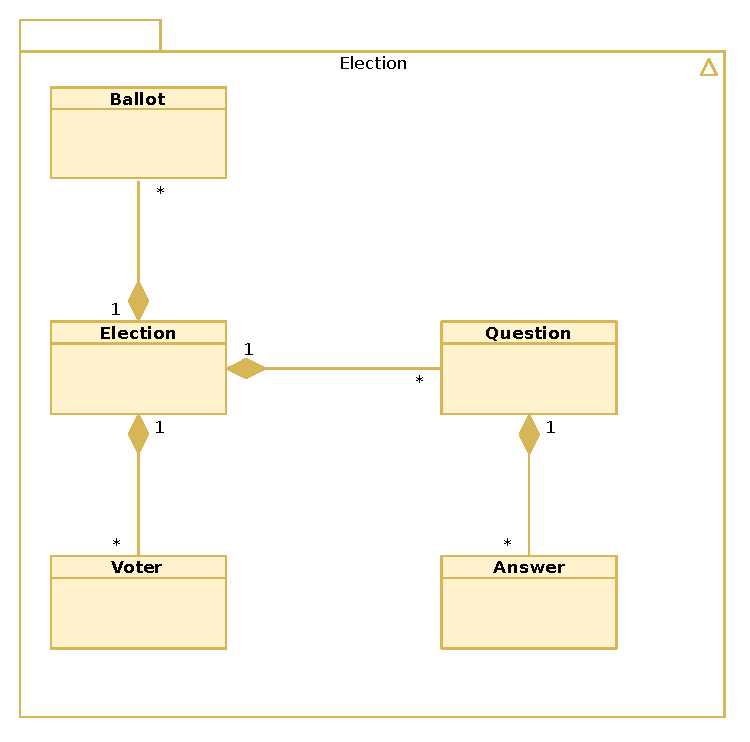
\includegraphics[width=0.6\linewidth]{svg/ElectionModelFull.eps}
	\captionsetup{width=0.6\linewidth}
	\caption[Model objektů balíčku Election]{Model objektů balíčku Election \\(zdroj: vlastní)}
	\label{fig:ElectionModel}
\end{figure}

Druhou zásadní částí aplikace je systém pro správu přístupu uživatelů (ACL). Nejjednodušší implementací takového systému je přiřazení oprávnění pomocí statické konfigurace. Tento přístup podporuje Nette bez nutnosti jakéhokoli dalšího rozšiřování o vlastní správu oprávnění. Nicméně takový přístup značně limituje flexibilitu aplikace, jelikož se jakákoli změna musí ručně zapsat do konfigurace, která bývá většinou uložena na serveru ve formě souboru. Z tohoto důvodu byl namodelován vlastní ACL systém.

\begin{figure}[h]
	\centering
	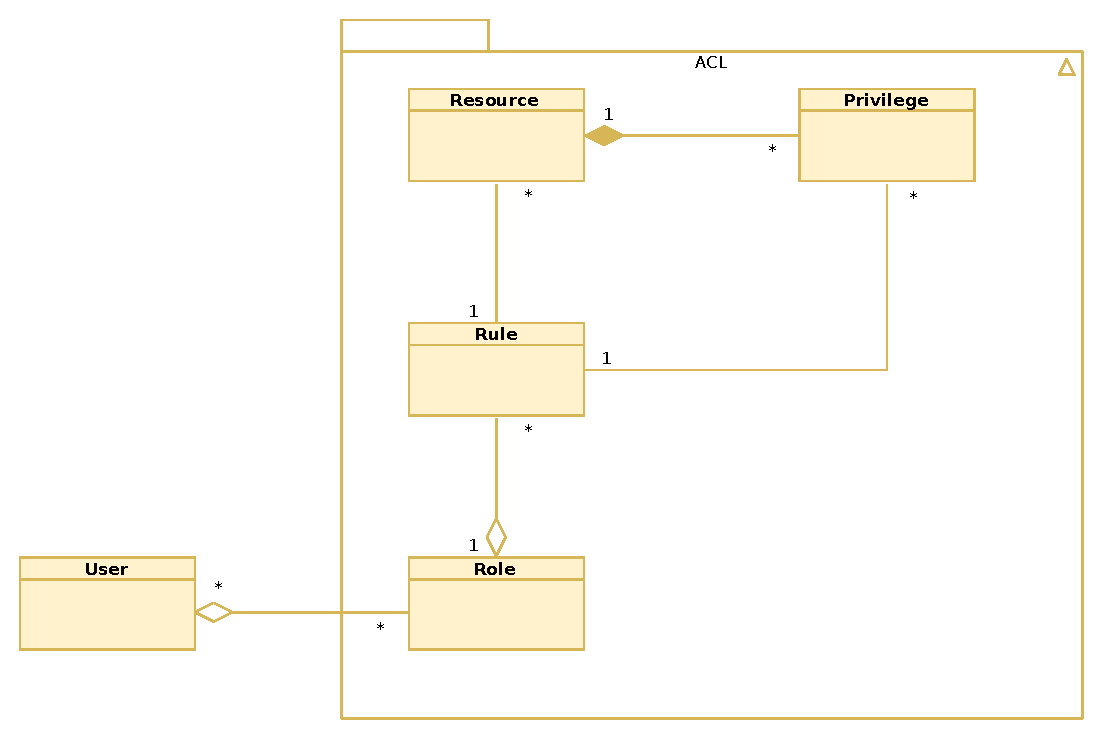
\includegraphics[width=\linewidth]{svg/ACLModelFull.eps}
	\captionsetup{width=\linewidth}
	\caption[Model objektů balíčku ACL]{Model objektů balíčku ACL (zdroj: vlastní)}
	\label{fig:AclModel}
\end{figure}
V tomto případě je kořenem agregátu entita \phpinline{Role} symbolizující jednu roli uživatele. Role může mít nastavena pravidla \phpinline{Rule}, která budou řídit přístup k~prostředkům \phpinline{Resource} a akcím \phpinline{Privilege} na nich vykonávaných. Každé pravidlo je kombinací právě jednoho prostředku a jedné akce. Pravidlo zároveň určuje, jestli je pro danou roli tato akce povolena nebo zakázána (\it{allow / deny}). Tabulka \ref{tab:prikladyACL} ukazuje příklady možného nastavení tohoto systému.


% \tab{popisek}{label}{rozměr (0.0 - 1.0)}{definice sloupců}{obsah} 
\tab{Příklady nastavení ACL}{tab:prikladyACL}{1}{llll}{
	\hline
	Role & Prostředek & Akce & Pravidlo \\
	\hline
	Student			&		Election		&		View		&	allow		\\
	Student			&		Election		&		Vote		&	allow		\\
	Student			&		Election		&		Delete	&	\bf{deny}\\
	Komise			&		Election		&		Count		&	allow		\\
	Administrator	&		Election		&		Activate	&	allow		\\
	SuperAdmin		&		User			&		Create	&	allow		\\
	\hline
}
\clearpage


\n{2}{Průchod voliče webem}
Jako další byl vytvořen zjednodušený případ užití celého systému, podle stanovanených požadavků, především s ohledem na zvolený systém anonymizace hlasovacích lístků, tak jak byl popsán v kapitole \koment{odkaz na kapitolu}.

\begin{figure}[h]
		\centering \tiny \fontfamily{lmss}\selectfont
		\def\svgwidth{1\columnwidth}
		\input{svg/ElectionUseCase2.pdf_tex}
		\normalsize \sffamily
		\captionsetup{width=\linewidth}
		\caption{Případ užití systému}
		\label{fig:UseCase}
\end{figure}

\cast{Praktická část}
\n{1}{Implementace návrhu}
Konkrétní implementace modelu popsaného v teoretické části probíhala postupně a vyvíjela se. Některé způsoby se po čase ukázaly jako nevhodné či nedokonalé a bylo potřeba je upravit resp. přepracovat tak, aby aplikace jako celek byla funkční. Během vývoje aplikace bylo změněno i IDE z Visual Studio Code na PHPstorm, což je místy vidět v rozdílných PHPdoc komentářích zdrojového kódu.

\n{2}{Členění aplikace}
Jednou ze změn, které se objevily jako vhodné v průběhu vývoje bylo rozdělení aplikace na dvě části, v kontextu Content Management Systémů běžně označované jako Frontend a Backend. Tyto dvě části by na sobě měly být nezávislé, tedy jedna nepotřebuje vědět o~(ne)existenci té druhé a umí svoje úkoly provést zcela samostatně. Frontend představuje tu část, která je veřejně dostupná, Backend označuje neveřejné administrační rozhraní aplikace. Tohoto rozdělení se zároveň využilo ke zvýšení bezpečnosti aplikace, jak je vysvětleno v části \ref{section:fyzickeOddeleni}.

Zjednodušená adresářová struktura je zobrazena v příloze \ref{priloha:adresare}. V adresáři \phpinline{app/} se nachází zdrojové kódy rozdělené podle jejich účelu. Presentery jsou společně se šablonami v příslušných adresářích (Backend, Frontend a Core). Core obsahuje presentery společné pro Frontend i Backend, což jsou momentálně pouze presentery pro zpracování chybových hlášení. Jednotlivé adresáře jsou popsány níže.
\begin{itemize}
	\item  \textbf{Backend} - obsahuje Presentery, šablony a pomocné třídy využité v Backendové části
	\item \textbf{Config} - konfigurační soubory aplikace
	\item \textbf{Core} - obsahuje Presentery, šablony a pomocné třídy využité napříč celou aplikací
	\item \textbf{Forms} - definice a továrny pro složitější formuláře
	\item \textbf{Frontend} - obsahuje Presentery a šablony využité ve Frontendové části
	\item \textbf{Models} - obsahuje modelovou vrstvu
	\item \textbf{Repositories} - všechny repozitáře pro komunikaci s modelovou vrstvou
	\item \textbf{Router} - definice routování
\end{itemize}

\n{3}{Fyzické oddělení} \label{section:fyzickeOddeleni}
Prvním krokem zabezpečení neveřejné části webu je samozřejmě omezení přístupu heslem přímo v aplikaci. Přihlašovací formulář je nicméně stále veřejný a kdokoli s~odkazem na přihlašovací stránku se může pokoušet o přihlášení. Druhým krokem tedy může být omezení přístupu pomocí IP adres (například pouze na adresy vnitřní sítě UTB) a to pomocí nastavení HTTP serveru souborem \tt{.htaccess} nebo v~konfiguraci \tt{virtualhost}. Toto nastavení je přenecháno ke zvážení tomu, kdo bude zodpovědný za instalaci a nastavení serveru.

Aby veškeré odkazy v aplikaci fungovaly a aby Nette vědělo kam má směřovat požadavky, bylo potřeba upravit základní routování popsané v části \ref{section:routovani}. Routy podporují tzv. moduly, které slouží přesně k takovému rozdělení aplikace na několik oddělených částí. Pro každý modul je možné definovat vlastní routy, seskupení rout do modulů se provádí voláním metody \phpinline{withModule(string $module)} %$ 
třídy \phpinline{RouteList}. 

\begin{listing}[ht]
\phpsnippet{tex/code/newRoute.php}
\caption{Upravená routa v Nette}
\label{php:newRoute}
\end{listing}

Rozšířené nastavení routování je patrné z fragmentu \ref{php:newRoute}. Obsahuje nastavení pro lokální testování (admin.volby.l) i simulaci produkčního prostředí na VPS serveru v~internetu (admin.volby.lukasrichter.eu). Pro Backendový modul bylo potřeba rozlišit jednotlivá prostředí podle názvu serveru kvůli použití domény čtvrtého řádu, se kterou si Router neporadil. Pro Frontendový modul toto nebylo potřeba, doména třetího řádu (volby.lukasrichter.eu) fungovala v pořádku. Zápis \phpinline{addRoute('/prihlasit', 'Sign:in')} definuje alias pro akci \tt{in} presenteru \tt{SignPresenter}, která je standardně dostupná pod adresou \tt{/sign/in}.

S tímto nastavením jsou jednotlivé části aplikace dostupné ze samostaných domén (např. admin.volby.utb.cz a volby.utb.cz), které nemusí být fyzicky na stejném serveru. Právě toto dokáže podstatně zvýšit bezpečnost aplikace. Frontendová část (volby.utb.cz) je umístěna na bežném veřejně přístupném serveru, zatímco Backendová část je umístěna na serveru, který nemusí být vůbec dostupný z~internetu. Samozřejmě může být rozdílná i samotná doména nižšího řádu, za~předpokladu, že jsou správně nastaveny DNS záznamy.

A jelikož jsou obě části na sobě nezávislé, není nutné na veřejně dostupném Frontendu umisťovat Backendový kód, který obsahuje například zpracování, dešifrování a počítání odevzdaných hlasů, ale i aktivaci a mazání celých voleb. V~případě útoku na aplikaci s cílem kompromitovat nebo ovlivnit volby, nemají útočníci možnost tento kód spustit. Museli by tedy útočit přímo na databázový server, jehož zabezpečení je v komptenci administrátora serveru.
\clearpage

\n{1}{Doménová vrstva}
Celý proces získání konkrétní entity pro potřeby aplikační vrstvy je postaven na~několika návrhových vzorech. Správné užití návrhových vzorů umožní zapouzdřit chování jednotlivých tříd, nebudou vytvářena těsná propojení jednotlivých tříd a celý zdrojový kód bude flexibilnější. Cílem tohoto přístupu je zjednodušení případných budoucích úprav aplikace. Těsné provázání tříd aplikační a databázové vrstvy sice znamená méně náročnou práci při první implementaci, ale o to je náročnější kód v~budoucnosti upravit. 

Příkladem může být objekt -- entita, který se umí perzistovat, tj. je přímo závislý na~konkrétní implementaci úložiště. Při změně úložiště je pak potřeba upravit všechny takové objekty.

\n{2}{Modelová vrstva}
Z pohledu architektury MVC reprezentuje modelová vrstva data a manipulaci s nimi a v aplikaci se výrazně překrývá s doménovou vrstvou z pohledu DDD. Způsob implementace byl zvolen tak, aby zbytek aplikace nebyl pevně spojen se způsobem získávání a ukládání dat (entit).

Single Responsibility Principle (Princip jedné odpovědnosti) zavedený Robertem~C.~Martinem udává, že ``třída by měla mít pouze jeden důvod ke změně''\footnote{A class should have only one reason to change\cite{Martin2002}}. Změnou je zde myšleno přepracování kódu. Pokud má třída pouze jednu odpovědnost, pouze ta může vyvolat nutnost změny kódu. Entita má odpovědnost podávat o sobě informace, její odpovědností není, jak je vytvořena, jak a jestli vůbec je perzistována v databázi či jinde atd. Vytváření entit by měla mít na starosti třída typu \phpinline{Factory}, převedení dat z~úložiště do formátu, kterému továrna rozumí je úkolem pro \phpinline{Data Mapper}. Získání entit pro potřeby aplikace je práce pro \phpinline{Repository}. 

Získávání a manipulace s entitami byla implementována pomocí návrhových vzorů Data Mapper a Repository. Aplikační vrstva (především Presentery) získává jako závislost repozitáře (třídy typu Repository), které jí poskytují požadované entity nebo kolekce entit. V souladu se SRP Presenter nezajímá, jakým způsobem jsou entity získávány, k jeho odpovědnosti to nepatří. Repozitáře vědí, že rozhraní Data mapper umí poskytovat entity bez ohledu na to, kde a jak je konkrétní entita uložena (v paměti, souboru, databázi či jinde). V aplikaci je pouze jedna implementace a to \phpinline{DbDataMapper}. Data mapper pomocí databázového adaptéru Dibi odesílá požadavky na databázový server. Vytváření entit je řešeno částečně továrními metodami data mapperů a částečně samotnými továrními třídami v závislosti na složitosti operace. Ideální by ovšem bylo striktní oddělení do samostatných tříd.

\begin{figure}[h]
	\centering
	\includegraphics[width=\linewidth]{svg/roleMapper.png}
	\captionsetup{width=\linewidth}
	\caption[Diagram modelové vrstvy]{Diagram modelové vrstvy (zdroj: vlastní)}
	\label{fig:RoleMapper}
\end{figure}

Diagram na obrázku \ref{fig:RoleMapper} obecně popisuje použité řešení, které bylo aplikováno na všechny entity. Třída \phpinline{RoleDbMapper} implementuje rozhraní \phpinline{RoleMapper}, které je předáno třídě \phpinline{RoleRepository} jako závislost. V diagramu je použit příklad role, vyhledat ji lze podle id nebo podle vazby na entitu \phpinline{User}. Vhodné například, pokud chceme zjistit, které konkrétní role má uživatel nastaveny a tedy k jakým prostředkům a akcím má přístup díky pravidlům přiřazeným k jeho daným rolím. Zde je vhodné připomenout diagram na obrázku \ref{fig:AclModel}, který popisuje vazby mezi uživatelem, rolemi atd.

Metody \phpinline{find(), findOne(), findAll()} a \phpinline{findRelated()} slouží k vyhledání entit podle zadaných parametrů. Těmi může být filtr na Id nebo společnou vlastnost ale i vazba na jinou entitu. Metoda \phpinline{getDataSource()} slouží k získání dat pro zobrazení interaktivních tabulek v administraci aplikace. Pomocí metody \phpinline{create()} dokáže vytvořit nové instance entity \phpinline{Role}, které jsou následně předány repozitáři samostatně (\phpinline{findOne()}) nebo jako kolekce (některé mappery předávají objekt \phpinline{...Collection}, některé předávají pole objektů).
\clearpage

\n{2}{Struktura databáze}
Pomocí stanovených modelů bylo možné navrhnout podrobnější modely jednotlivých entit a tím pádem i strukturu databáze.

\begin{figure}[h]
	\centering
	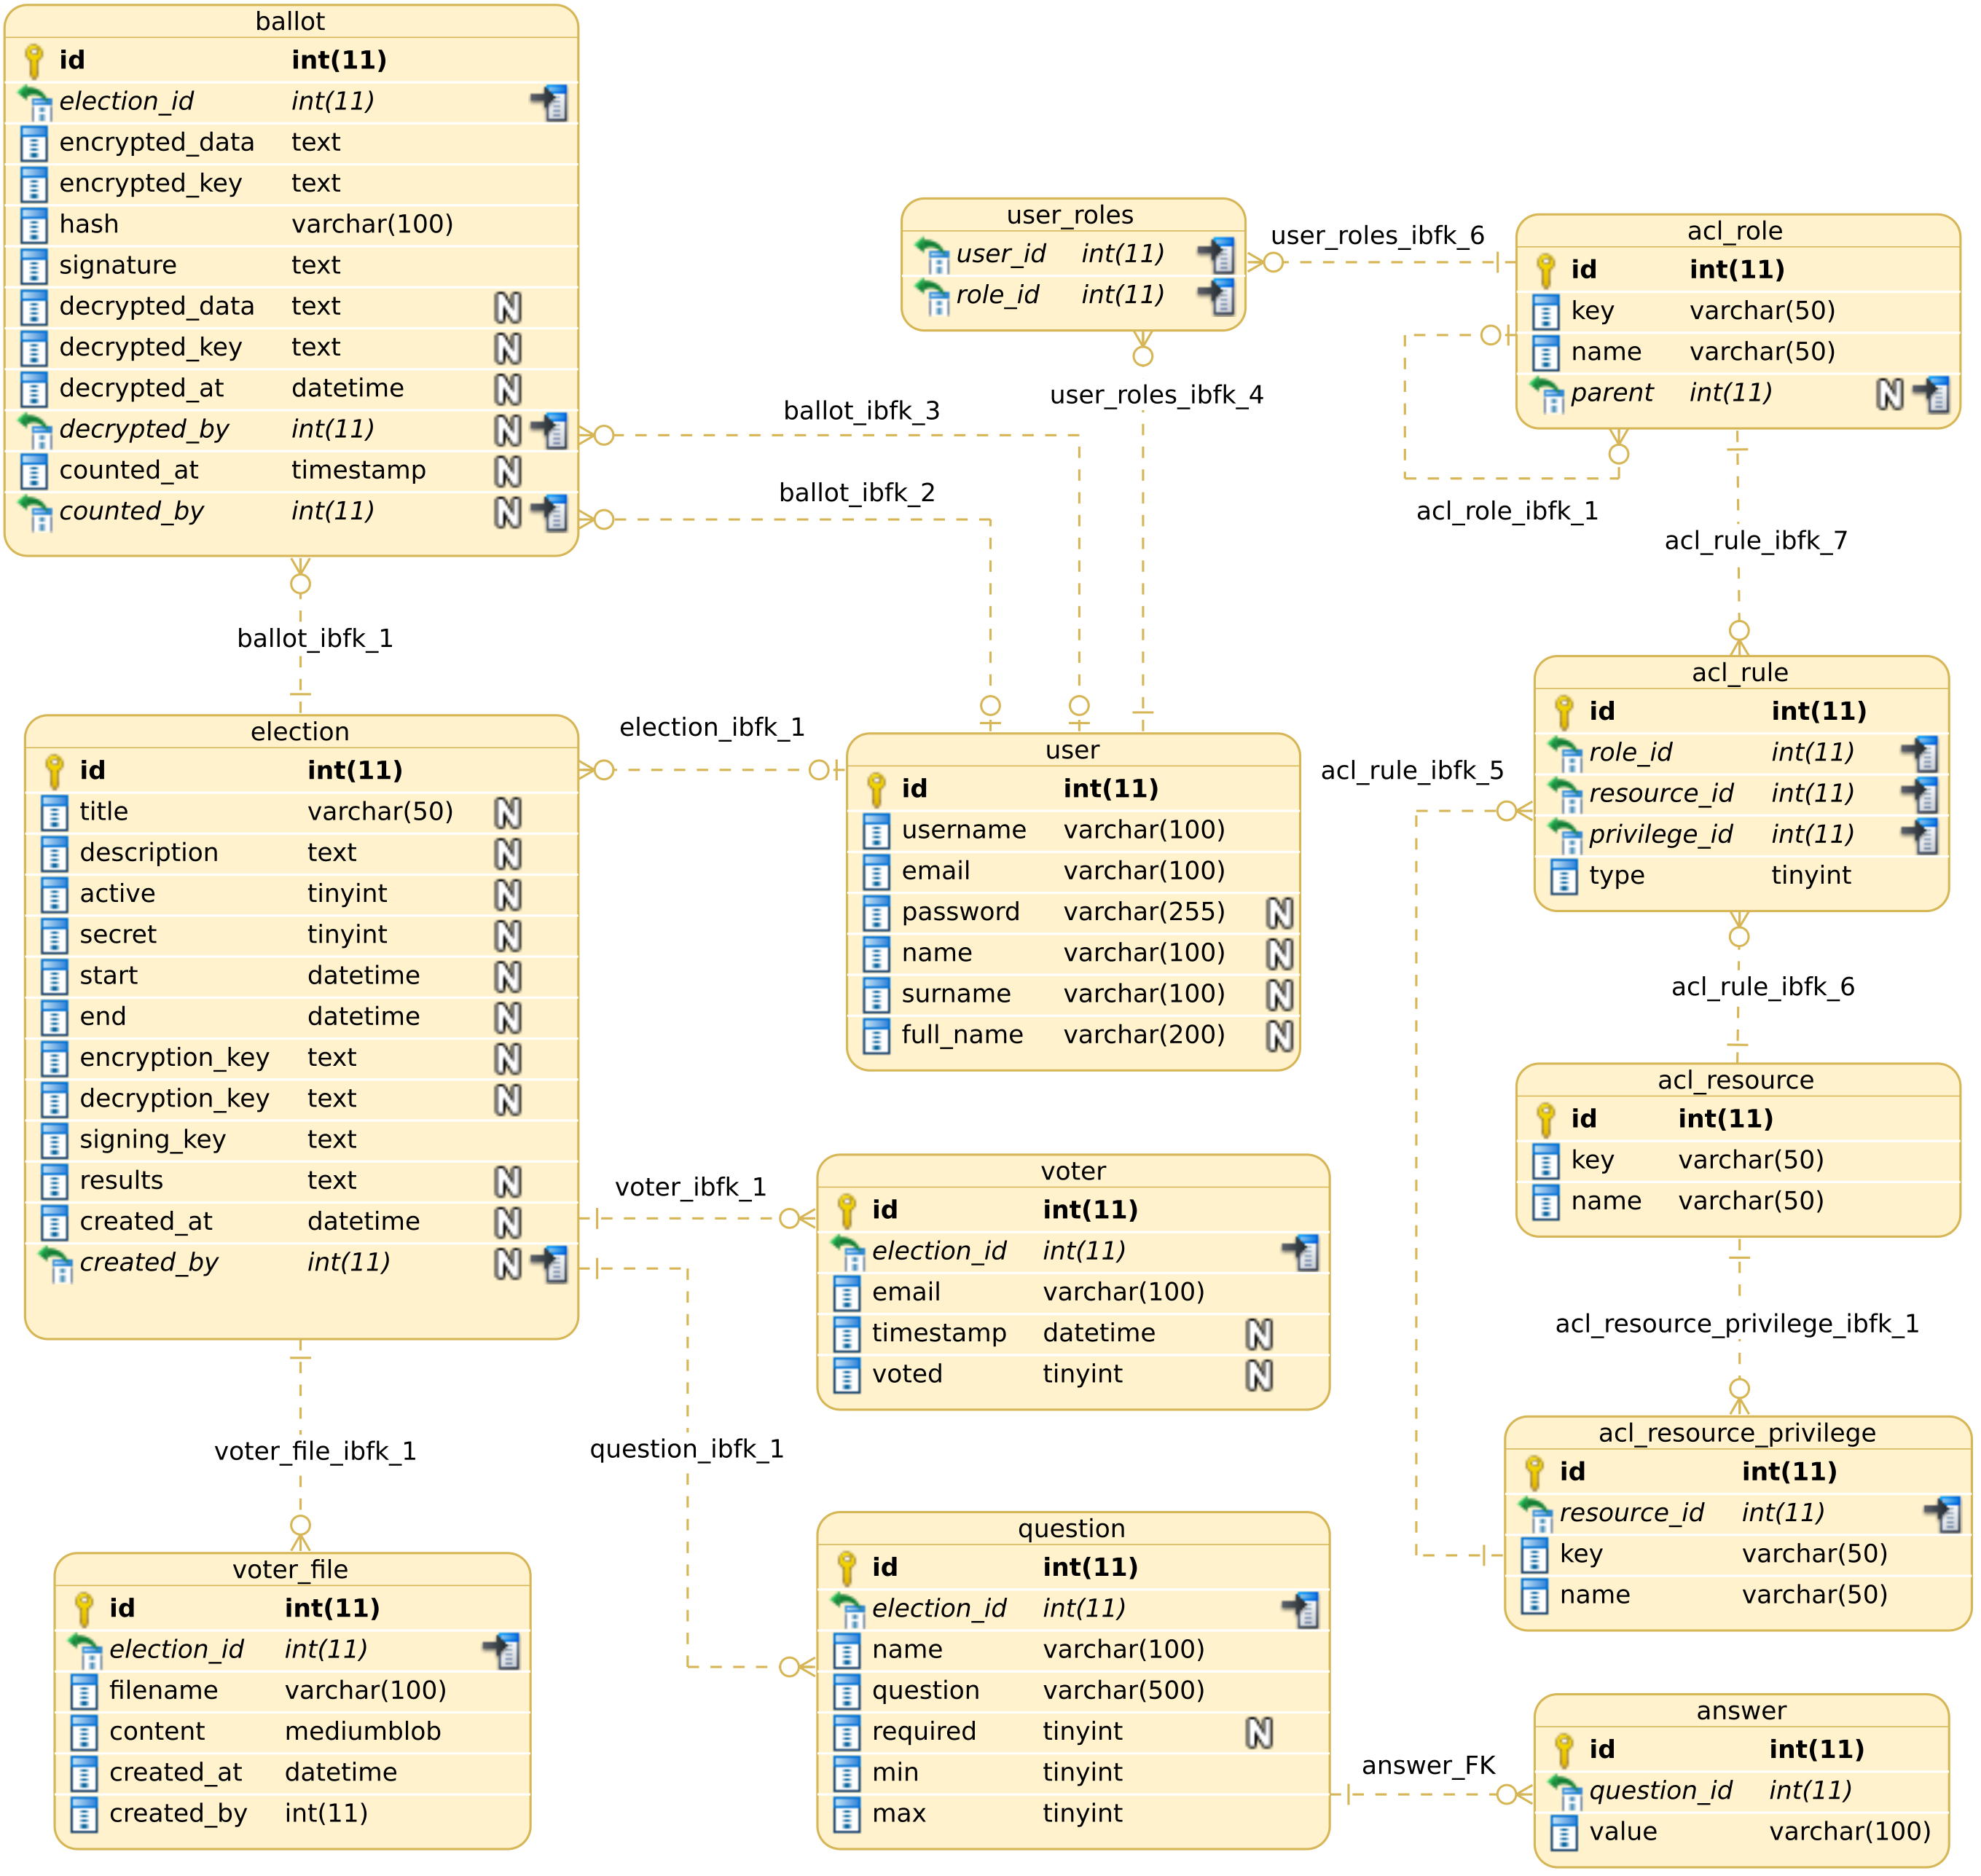
\includegraphics[width=\linewidth]{svg/erd3.png}
	\captionsetup{width=\linewidth}
	\caption[Entitně relační diagram]{Entitně relační diagram (zdroj: vlastní)}
	\label{fig:ERD}
\end{figure}


\clearpage

\n{1}{Vrstva infrastruktury}

\n{2}{Přihlašovaní a autentizace} \label{section:prihlasovani}
Přihlašování uživatelů probíhá identickým způsobem pro Frontend i Backend. Aplikace je dostupná pouze pro přihlášené, pokus o přístup bez platného přihlášení vyvolá přesměrování na SignPresenter. Přestože základní URL adresa aplikace vede na \texttt{Homepage:default}, (nepřihlášení) uživatelé jsou vždy přesměrováni nejdříve na přihlašovací stránku.

K ověření (autentizaci) uživatele pomocí kombinace uživatelského jména (e-mailové adresy) a hesla v Nette slouží rozhraní \texttt{Authenticator}\footnote{\Verb{Nette\Security\Authenticator}}. Samotný proces ověření inicializuje objekt \texttt{User}\footnote{\label{user}\Verb{Nette\Security\User}}. SignPresenter po odeslání formuláře předá objektu \texttt{User} implementaci rozhraní a následně zavolá metodu \phpinline{User::login($username, $password)}. Pokud ověření selže, je vyvolána výjimka \texttt{AuthenticationException}, která je zachycena v presenteru. Úspěšná autentizace způsobí uložení implementace \texttt{IIdentity} do objektu \texttt{User}.

Jedním z požadavků na aplikaci byla stanovena možnost přihlášení voličů pomocí univerzitních e-mailových adres. Implementace ověřování metodou Single Sign-On přes systém Shibboleth by byla nad rámec této práce a po diskuzi s vedoucím práce bylo zvoleno ověřování pomocí Active Directory přes LDAP. Dalším požadavkem byla možnost přihlášení externích uživatelů bez nutnosti vytvářet jim univerzitní e-mailové adresy. Tohoto bylo docíleno možností ověření vůči databázi aplikace.

\begin{listing}[ht]
\phpsnippet{tex/code/autentizace.php}
\caption{Autentizace v SignPresenter}
\label{php:autentizace}
\end{listing}

K autentizaci se využívají dvě implementace třídy \texttt{Authenticator}. První se k ověření použije \texttt{PasswordAuthenticator}, která při úspěšném ověření vrací entitu uživatele včetně všech rolí, při neúspěchu následuje pokus o ověření přes \texttt{LdapAuthenticator}.

\begin{itemize}
	\item \textbf{PasswordAuthenticator} v prvním kroku získá na základě e-mailové adresy entitu uživatele z repozitáře. Pokud takový uživatel v databázi není, je vyvolána výjimka \texttt{AuthenticationException}. V druhém kroku předá uloženou hash hesla a ověřované heslo třídě \phpinline{Nette\Security\Passwords} k porovnání. Pokud heslo neodpovídá, je opět vyvolána výjimka. Úspěšné ověření vrátí získanou entitu.
	\item \textbf{LdapAuthenticator} v prvním kroku se pokusí ověřit kombinaci e-mailové adresy a hesla vůči univerzitnímu Active Directory, při neúspěchu vyvolá výjimku. V druhém kroku se pokusí získat z repozitáře entitu uživatele s odpovídající e-mailovou adresou, pokud takový neexistuje, je vytvořena nová entita s rolemi získanými z Active Directory. Tyto role jsou buď \textit{Student} nebo \textit{Zaměstnanec}.
\end{itemize}



\clearpage
\n{2}{Oprávnění a autorizace}
Ověření oprávnění uživatele provést akci (autorizace) na frontendové části je velice přímočaré. Zobrazit přehled aktivních voleb může kdokoli úspěšně autentizovaný systémem. Volit a zobrazit výsledky může kdokoli, kdo je uveden na seznamu voličů. Není třeba provádět žádnou dodatečnou autorizaci operací.

Backendová část je v tomto ohledu o něco složitější. Jednotliví uživatelé mohou mít přístup k presenteru, ale už ne k nějaké jeho konkrétní akci nebo signálu (metodám obecně). Podle modelu definovaného v části \ref{section:Entity} byly vytvořeny jednotlivé třídy entit. Proces autorizace stejně jako autentizace inicializuje Nette objekt \texttt{User}\footnote{\label{user}\Verb{Nette\Security\User}}. V případě přihlašování uživatelů jsou mu předávány implementace napřímo, jelikož se používají dvě různé. U autorizace stačí předat jednu konkrétní implementaci, což je nejjednodušší provést v konfiguračním souboru aplikace. V soubrou \texttt{common.neon} tedy byly zaregistrovány služby \texttt{Permission}\footnote{\Verb{Nette\Security\Permission}} a \texttt{AuthorizatorFactory}. Framework se o předání závislostí postará sám.

V rámci třídy \texttt{AuthorizatorFactory} jsou z repozitáře získány včechny prostředky a jejich akce a zaregistrovány v \texttt{Permission}. Dále se získají všechny role a postupně se zaregistrují společně s jejich pravidly. Jako poslední je zaregistrována role \textit{superAdmin}, uživatel s touto rolí má nastaveno jediné pravidlo - vše povoleno. 

\begin{listing}[ht]
\phpsnippet{tex/code/autorizace.php}
\caption{Tovární metoda třídy AuthorizatorFactory}
\label{php:autorizace}
\end{listing}

Nette umožňuje pravidla nastavovat dvojím způsobem, výčtem povolených akcí a~povolením všech akcí a výčtem akcí zakázaných. Aplikace umožňuje vytvořit pravidla obou typů, zakazující (deny) typ má nicméně smysl pouze pro roli superAdmin, která je jako jediná definována druhým způsobem. Ostatní role vždy obsahují pouze výčet povolených akcí, vše ostatní je zakázáno.

Zjistit, zda je uživatel oprávněn provést požadovanou akci, lze několika způsoby. Napřímo pomocí metody \phpinline{User::isAllowed($resource, $privilege)}, která vrací \texttt{true}, pokud alespoň jedna z rolí uživatele k akci opravňuje, jinak vrací \texttt{false}. Tento způsob lze využít i v šablonách, kde je objekt uživatele automagicky [\textit{sic}] dostupný jako proměnná \phpinline{$user}%$
. V presenterech se získá pomocí \phpinline{$this->getUser()} %$
 a~komponenty mají presenter dostupný jako členskou proměnnou, objekt \texttt{User} tedy získají pomocí \phpinline{$this->presenter->getUser()}%$
. Ostatním třídám aplikace se předává jako závislost v konstruktoru pomocí DI Containeru.

Jelikož presentery zpracovávají především požadavky od uživatele, podstatná část jejich metod by obsahovala opakující se volání metody \texttt{isAllowed}. Proto bylo využito anotací jednotlivých metod, příklad takové anotace je uveden ve fragmentu \ref{php:autorizaceAnotace}. Čtení anotací Nette usnadňuje pomocí objektu \texttt{MethodReflection}\footnote{\Verb{Nette\Application\UI\MethodReflection}}, který je předáván metodě \texttt{checkRequirements()} každého presenteru. Tato metoda je v průběhu životního cyklu presenteru volána několikrát, poprvé při jeho vytvoření a předává se jí objekt \texttt{ComponentReflection}\footnote{\Verb{Nette\Application\UI\ComponentReflection}} - reflexe aktuálního presenteru - a poté před každým \textit{action}, \textit{handle} a \textit{render} v tomto pořadí s reflexí dané metody. Tímto bylo dosaženo velice efektivního zabezpeční jednotlivých částí presenteru.

\begin{listing}[ht]
\phpsnippet{tex/code/anotace.php}
\caption{Příklad anotace metody}
\label{php:autorizaceAnotace}
\end{listing}

\clearpage
Zpracování anotací probíhá v abstraktním presenteru \texttt{BasePresenter}. Pokud uživatel nedisponuje patřičným oprávněním, je mu zobrazena varovná zpráva (\textit{flashMessage}) a je přesměrován na výchozí \textit{View} aktuálního presenteru, pokud nemá oprávnění ani k tomu, je přesměrován na \texttt{HomepagePresenter}.

\begin{listing}[ht]
\phpsnippet{tex/code/checkRequirements.php}
\caption{Autorizace pomocí anotací metod}
\label{php:autorizaceCheckRequirements}
\end{listing}

\n{1}{Aplikační a prezentační vrstva}
Aplikační vrstva je tvořena především presentery, které obsluhují požadavky uživatele a pomocné třídy.  Ty mohou být zcela samostatné nebo rozšiřují chování využívaných Composer balíčků. Prezentační vrstva je tvořena šablonami. Použitá architektura propojuje a částečně prolíná obě vrstvy, proto jsou uváděny společně. Toto prolínání podle Davida Grudla vidíme i v Nette, jak uvádí v komentáři u svého článku: ,,Dalo by se říct, že metoda \texttt{renderDefault()} je součástí vrstvy View, společně se šablonou.'' \cite{NetteRefactoring}

\n{2}{Presentery}
V aplikaci se nachází tři skupiny presnterů, podle příslušnosti k modulu: Core, Backend a Frontend. Šablony pro konkrétní Presenter jsou ve společném adresáři \tt{templates/jmenoPresenteru/} a název souboru každé šablony odpovídá akci daného presenteru. Pokud akce nevede na vykreslení šablony, nemusí mít šablonu vůbec vytvořenou. Příkladem je \tt{Sign:out} (\it{SignPresenter} a akce \it{out}), která přihlášeného uživatele odhlásí a přesměruje na přihlašovací formulář \tt{Sign:in} (stejný presenter, akce \textit{In}). SignPresenter obsahuje metodu \phpinline{renderIn} a tedy vyžaduje i šablonu \tt{templates/Sign/in.latte}

%--------------%
%--------------%

\n{3}{Frontend}
\begin{figure}[h]
	\centering
	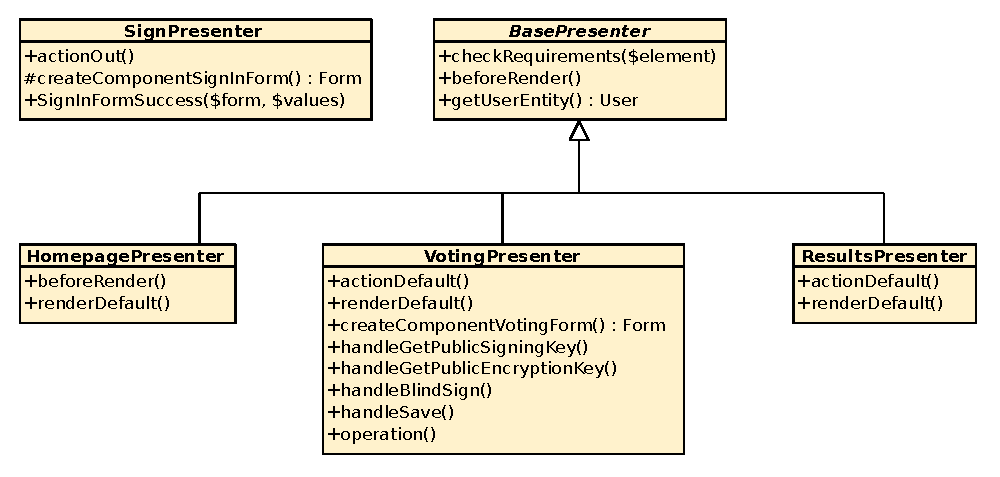
\includegraphics[width=\linewidth]{svg/frontendPresenters.eps}
	\captionsetup{width=\linewidth}
	\caption[Třídy Presenter frontendové části]{Třídy Presenter frontendové části (zdroj: vlastní)}
	\label{fig:FrontendPresenters}
\end{figure}
%--------------%
\clearpage
\paragraph{SignPresenter} Jediným úkolem tohoto presenteru je uživateli poskytnout možnosti přihlášení a odhlášení.

% \tab{popisek}{label}{rozměr (0.0 - 1.0)}{definice sloupců}{obsah} 
\tab{Dostupné akce}{tab:FrontendSignPresenterAction}{1}{c|ccc}{
	\hline
	akce & action* & render* & šablona \\
	\hline
	in & - & - & in.latte \\
	out & actionOut & - & - \\
}

Dostupné akce:
\begin{itemize}
	\item \tt{Sign:in} Zobrazí přihlašovací formulář\\
Nemá definované metody action ani render - ekvivalentní by byly prázdné metody. Jediným úkolem této metody je zobrazit formulář pro přihlášení, který se vytváří metodou \phpinline{SignPresenter::createComponentSignInForm()}. Po~odeslání formuláře se volá opět tato akce, nicméně se provede i callback formuláře \phpinline{SignPresenter::signInFormSuccess()}. V tomto callbacku se aplikace pokusí o přihlášení uživatele pomocí poskytnutých údajů. Presenter je předá třídě implementující rozhraní \phpinline{Nette\Security\IAuthenticator}. Princip přihlašování je popsán v části \ref{section:prihlasovani}. Na tuto akci zároveň odkazují všichni potomci BasePresenter z metody \phpinline{BasePresenter::checkRequirements()}, pokud se uživatel pokusí provést jakoukoli akci jako nepřihlášený (např. po~vypršení session).
	\item \tt{Sign:out} Odhlásí uživatele\\
Uživatel po kliknutí na odkaz ,,Odhlásit'' vyvolá akci tuto akci, kdy je odhlášen a následně přesměrován na přihlašovací formulář -- \tt{Sign:in}. Tato akce nemá render metodu ani šablonu (dochází k přesměrování, které předchází jakémukoli výstupu a ukončuje aktuální cyklus aplikace).
\end{itemize}


%--------------%
\paragraph{BasePresenter} je abstraktní třída, která je společným předkem pro všechny presentery, které jsou dostupné pouze po přihlášení. Také obsahuje metody, které jsou užitečné pro všechny presentery obecně. Vzhledem k tomu, že se jedná o abstraktní presenter, nemá žádné metody action, render ani vlastní šablony. 
Metoda \phpinline{checkRequirements()} slouží k ověření, že je uživatel přihlášen. Rozšiřuje rodičovskou metodu, která detekuje CSRF\footnote{Cross-Site Request Forgery} útoky, je tedy nezbytné zahrnout \phpinline{parent::checkRequirements($element)}%$
. Aby bylo zajištěno správné zobrazení krátkých stavových zpráv \it{flashMessage} a modálních oken během AJAXových požadavků, je zde i metoda \phpinline{beforeRender()}, která se volá vždy před metodami \phpinline{render}.


%--------------%
\paragraph{HomePagePresenter} slouží jako rozcestník po přihlášení uživatele. Jeho jediná akce je \texttt{Homepage:default}, a obsahuje pouze render metodu, která získává objekty Election, které jsou dostupné danému uživateli.


%--------------%
\paragraph{VotingPresenter} je stěžejním presenterem frontendové části aplikace, jejímž prostřednictvím probíhá celý proces volby na straně uživatele. Metoda \phpinline{actionDefault()} získává a \phpinline{renderDefault()}  předává šabloně objekt \phpinline{Election}. Samotný hlasovací lístek je tvořen formulářem. Ten je vytvářen tovární metodou \phpinline{createComponentVotingForm()}. Zde bylo využito \it{generované továrničky}, což je zjednodušený zápis továrních tříd, které pouze vytváří jeden konkrétní objekt. Do~presenteru je pomocí Dependency Injection předána závislost na rozhraní \phpinline{VotingFormFactory} a Nette samo vygeneruje implementaci tohoto rozhraní, které je předáno do Presenteru \cite{Planette}.

Formulář \phpinline{VotingForm} je samostatnou třídou rošiřující \phpinline{Control}\footnote{\Verb{Nette\Application\UI\Control}} - v názvosloví Nette komponentou. Komponenty mohou mít vlastní šablony, což umžňuje zpřehlednit šablonu presenteru pokud není celý formulář vykreslován automaticky přes \phpinline{FormRenderer}. Zároveň je i samotný kód presenteru jednodušší, o vytvoření formuláře, validaci a zpracování se totiž stará třída formuláře.

Hlasovací formulář neobsahuje žádnou logiku pro validaci ani zpracování odeslaných dat. Veškerá validace probíhá pomocí JavaScriptu na straně klienta a data se odesílají teprve po zašifrování a to přímo na presenter pomocí AJAX. Zpracování těchto požadavků (signálů) pomocí handle metod je popsáno v samostatné části~\ref{section:zpracovaniHlasu}~věnované zpracování hlasovacích lístků.


%--------------%
\paragraph{ResultsPresenter} je velice jednoduchý presenter, který opět pomocí metod \phpinline{actionDefault()} a \phpinline{renderDefault()} získá a zpřístupní objekt \phpinline{Election} šabloně k~zobrazení výsledků hlasování / voleb.

%--------------%
%--------------%
\n{3}{Backend}

Tato část obsahuje nástroje pro správu uživatelů, uživatelských oprávnění a~především voleb samotných. Je hojně využíváno formulářů a interaktivních tabulek (neboli datagridů). Formuláře a datagridy jsou samostatné komponenty\footnote{třídy rozšiřující \phpinline{Nette\Application\UI\Control}}. Jednoduché komponenty jsou zpravidla vytvářeny přímo v Presenteru. Složitější chování nebo obsáhlé komponenty je vhodnější oddělit do samostatné třídy. Podrobněji jsou datagridy popsány v části \ref{section:Datagridy}.

Datagridy jsou vytvářeny pomocí třídy \phpinline{App\Backend\Utils\DataGrid\Datagrid}, která zefektivňuje způsob vytváření jednotlivých gridů díky zapouzdření často používaných konstrukcí. Tím se nejen výsledný kód v presenterech zjednoduší, ale zároveň gridy napříč aplikací mají stejné chování a na všechny se aplikuje stejná logika. Tímto přístupem se také podstatně usnadní změny ovlivňující všechny gridy - například změna ikony se projeví všude.

\begin{figure}[h]
	\centering
	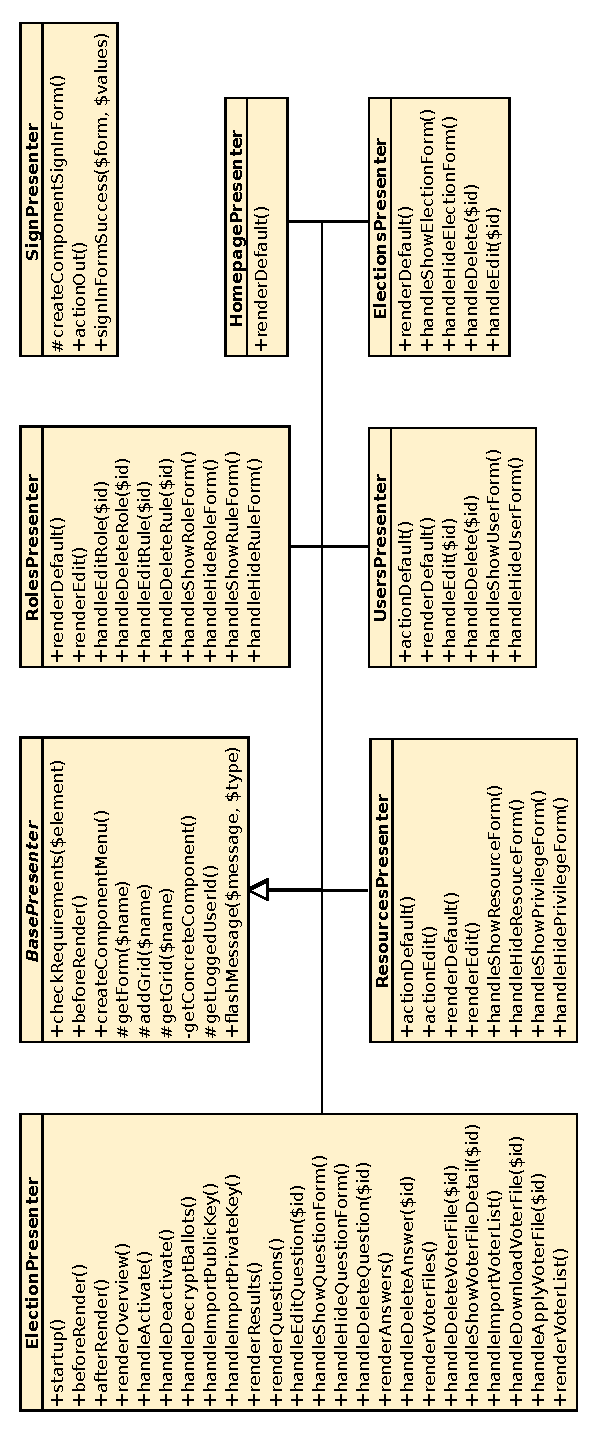
\includegraphics[height=\textheight]{svg/backendPresentersPortrait.eps}
	\captionsetup{width=\linewidth}
	\caption[Třídy Presenter backendové části]{Třídy Presenter backendové části (zdroj: vlastní)}
	\label{fig:BackendPresenters}
\end{figure}

%--------------%
\paragraph{SignPresenter} slouží ke správě přihlášení do aplikace, v zásadě se jedná o obdobu frontendového \phpinline{SignPresenter}. Popis této třídy je tedy identický.


%--------------%
\paragraph{BasePresenter} je stejně jako \phpinline{App\Frontend\Presenters\BasePresenter} abstraktní třídou společnou pro všechny další presentery. Ověřuje, že uživatel je přihlášen a má oprávnění provést požadovanou akci.


%--------------%
\paragraph{HomepagePresenter} hlavní jeho funkcí je umožnit zobrazení navigace po přihlášení i pro uživatele, který nemá definovaná žádná práva a jediné co může v aplikaci provést je se odhlásit. Mohl by zobrazovat i nějakou formu rozcestníku, jako ve frontendové části, to ale obstarává navigační lišta. Dalším vhodným využitím tohoto presenteru by byla prezentace důležitých dat formou \it{dashboardu}.


%--------------%
\paragraph{ElectionsPresenter} poskytuje přehled nad všemi vypsanými volbami, jejich rychlou editaci, mazání a odkaz na zobrazení detailu. Nové volby se také vytváří v tomto presenteru. Při vypisování nových voleb je vhodné zvolit výstižný krátký popisek, jeho editace je uživatelsky přívětivá díky JavaScriptovému pluginu \it{tinyMCE}.


%--------------%
\paragraph{ElectionPresenter} nabízí detailní přehled konkrétních voleb rozdělený do záložek. Některé záložky se zobrazují pouze pokud se volby nacházejí v určitém stavu. Záložka výsledky se například zobrazí až po ukončení voleb. 

V záhlaví detailu se nachází kontextové menu, které umožňuje volby (de)aktivovat, nahrávat seznamy voličů a klíče volební komise. Aktivace voleb způsobí jejich zobrazení voličům, hlasování je umožněno až v řádném termínu. Po aktivaci voleb není možné měnit jejich nastavení, ale lze je opět deaktivovat. Aktivovat a deaktivovat volby lze pouze pokud se nenacházejí v průběhu jejich konání. Po skončení voleb se voličům ukazují pouze výsledky a to do doby než jsou deaktivovány.

Jednotlivými záložkami jsou:
\begin{itemize}
	\item \b{Overview}, kde se zobrazuje formátovaný popis voleb a tři pole s šifrovacími klíči (pokud jsou dostupné). Těmito klíči jsou: privátní a veřejný klíč volební komise a veřejný podpisový klíč serveru.
	\item \b{Results} s výsledky voleb. Tato záložka je distupná pouze po ukončení voleb. V~případě, že dosud nejsou spočítané výsledky, je nabídnuto jejich spočítání a~následně se již zobrazují pouze výsledky v přehledných grafech.
	\item \b{Questions} zobrazí grid otázek definovaných pro dané volby. Otázkou může být volená pozice, její odpověďmi pak jména kandidátů. Při založení nové otázky je možné nastavit minimální a maximální počet otázek, zda je odpověď povinná a~jednotlivé odpovědi. V gridu je možné otázky editovat a mazat.
	
	\item \b{Answers} obsahuje grid všech odpovědí, které byly definované při zakládání otázek, zde je možné odpovědi mazat.
	
	\item \b{Voter list} zobrazí grid s aktivním seznamem voličů.
	
	\item \b{Voter files} v tomto gridu se nachází všechny soubory se seznamem voličů, které byly pro dané volby nahrány. Soubory je možno prohlížet, mazat, stáhnout a~aplikovat vybraný soubor jako aktivní seznam voličů. Nový soubor lze nahrát přes kontextové menu v záhlaví.
	
\end{itemize}

%--------------%
\paragraph{UsersPresenter} jednoduchý presenter s gridem uživatelů a formulářem pro přidávání / editaci uživatelů. Formulář umožňuje uživatelům přidělovat role i změnit heslo. Aplikace neobsahuje žádný registrační formulář, nové uživatele musí vždy přidávat osoba s patřičným oprávněním - pravděpodobně administrátor aplikace. Jak bylo popsáno v části \ref{section:prihlasovani}, není potřeba zakládat uživatelské účty voličům, ale pouze osobám, kterým je potřeba navýšit oprávnění.

%--------------%
\paragraph{RolesPresenter} výchozí View tohoto presenteru nabízí grid všech dostupných rolí a~formulář pro jejich základní editaci. Pomocí akce gridu je možné zobrazit detail role, kde se nachází seznam definovaných pravidel přístupu ve formě gridu. Tato pravidla lze editovat, mazat a přidávat nová.

%--------------%
\paragraph{ResourcesPresenter} velice podobý předchozímu RolePresenter. Tento umožňuje správu prostředků (\textit{Resource}), na stránce detailu je pak k dispozici správa akcí (\textit{Privilege}) dostupných pro daný prostředek.

\n{3}{Core}
Tento modul je společný pro frontendovou i backendovou část a obsahuje pouze uživatelsky přívětivé zpracování chybových stavů. Pokud se uživatel pokouší přistoupit na neexistující stránku, není nalezen požadovaný záznam v databázi (HTTP~404) nebo nemá uživatel potřebná oprávnění k zobrazení stránky (HTTP~403), místo základních chybových stránek HTTP serveru mu je zobrazena chybová stránka vygenerovaná Nette. Stejně tak v případě chyby serveru (HTTP~500). 

V případě, že se Nette nachází ve vývojovém režimu, jsou všechny chyby aplikace předávány ke zpracování nástroji Tracy (dříve Laděnka) \cite{Tracy}, který vypíše chybu včetně části zdrojového kódu, předávaných proměnných, dotazů na databázi a dalších velice užitečných informací pro ladění chyb. V produkčním režimu jsou chyby předávány \texttt{ErrorPresenteru}, který chyby 4xx předává dále do \texttt{Error4xxPresenter} případně rovnou předá statickou šablonu s chybou 500 nebo 503.



\n{2}{Šablony}
Šablony (\textit{templates}) jsou součástí zobrazovací vrstvy (View) aplikace a jejich účelem je prezentovat uživateli data z aplikační a doménové vrstvy v lidské podobě. Pro jednoduchost popisu byly do této části zařazeny i kaskádové styly (CSS) a JavaScript (JS), přestože nejsou ve striktním podání šablonami.

Jak již bylo popsáno, šablona je těsně navázána na presenter a jeho akci. I pokud presenter nemá definované žádné metody akce (\texttt{action}, \texttt{render}), pokud existuje šablona, může být zobrazena. Každá šablona musí být umístěna v adresáři, který se shoduje s názvem presenteru a název souboru šablony musí odpovídat názvu akce. Prázdná (relativní) URL adresa webu směřuje na HomepagePresenter a jeho akci default. Pokud má existovat i výstup pro danou adresu, šablona \texttt{default.latte} bude umístěna do adresáře \texttt{templates/Homepage/}, přičemž adresář \texttt{templates} je na stejné úrovni jako adresář obsahující presentery.

Výstupem šablony je nejčastěji HTML kód zobrazený v prohlížeči. Nette umožňuje vykreslovat i samostatné části šablon zvané \textit{snippety} \cite{NetteDocs}, čehož je hojně využíváno pro AJAXové požadavky. Presenter po zpracování AJAX požadavku může jako odpověd poslat pouze část šablony ve formě JSON řetězce, který zpracuje JavaScriptová knihovna Naja a vloží na konkrétní místo v HTML dokumentu, který má prohlížeč již načtený. Tímto se podstatně snižuje objem přenesených dat, ale především rychlost načtení požadovaného obsahu. Na uživatele aplikace zároveň působí svižně, jelikož nedochází k překreslování celého obsahu prohlížečem, změní se pouze ta část dokumentu, která je definovná jako snippet.

Snippety jsou v aplikaci použity pro formuláře, datagridy a další. Detail konkrétních voleb obsahuje jednotlivé záložky, které také využívají snippetů a~AJAXových požadavků. Knihovna Naja navíc umí simulovat historii prohlížení i~změnou URL adresy v adresním řádku prohlížeče, zároveň funguje i možnost v~historii listovat pomocí příkazů \textit{zpět} a \textit{vpřed} prohlížeče.

\n{3}{CSS styly}
Aplikace využívá CSS frameworku Bootstrap původně vyvinutý ve společnosti Twitter a v současnosti jeden z nejpoužívanějších CSS frameworků vůbec \cite{Bootstrap}. Bootstrap umožňuje vytvářet responzivní stránky velice snadno pouze použitím CSS tříd. Použitá verze (Bootstrap v4.6) využívá \textit{flexbox} k dosažení responzivního vzhledu. Tento framework (a verze) byl zvolen vzhledem k dostupným rozšířením pro Nette formuláře a datagridy, které tak působí jednotným vzhledem. Některé formuláře musely být i tak vykresleny manuálně, aby bylo dosaženo požadovaného vzhledu, především kvůli nedokonalému zobrazení chyb ve formuláři.

Vlastní a upravené kaskádové styly jsou uloženy v \texttt{custom.css}, další používané CSS soubory jsou závislostmi používaných balíčků. V backendové části jsou také použity ikony FontAwesome \cite{FontAwesome}.

\n{3}{Skripty a balíčky}

Aplikace také využívá několik JavaScriptových knihoven a vlastních skriptů. Vlastními skripty jsou rozšíření pro knihovnu Naja a skript pro šifrování hlasů na straně klienta. Naja byla rozšířena o možnost nuceného přesměrování, indikaci načítání stránky při AJAXovém požadavku, zobrazení modálních oken a uložení obsahu editoru tinyMCE před odesláním formuláře na server.
\begin{itemize}
	\item Naja - obsluha a zpracování AJAX požadavků
	\item jQuery - knihovna pro manipulaci s Document Object Model (DOM)
	\item netteForms - validace formulářů
	\item Bootstrap - knihovna Bootstrap frameworku
	\item toastr.js - zobrazení krátkých stavových zpráv (toastů)
	\item charts.js - interaktivní grafy
	\item tinyMCE - WYSIWYG textový editor ve formulářových polích \texttt{textarea}
	\item SweetAlert2 - uživatelsky přívětivé upozornění a dialogová okna
\end{itemize}



\clearpage
\n{2}{Pomocné třídy}
%\begin{comment}
\n{3}{Datagridy} \label{section:Datagridy}
Zkráceně gridy, tyto interaktivní tabulky umožňují kromě zobrazení dat i jejich filtraci, stránkování, akce nad řádkem tabulky (např. odkaz směřující na \textit{Signál}) a mnoho dalších funkcí. Gridy přijímají data jako objekt \phpinline{Datasource}, který může obsahovat data ve formě obyčejného pole nebo dotazu SQL \cite{ContributteDataGrid}. Kromě jednoho případu v této aplikaci vždy pracují s SQL dotazem. Výhoda tohoto přístupu je minimalizování potřebného objemu dat k zobrazení gridu. Po změně filtrace nebo stránky je vždy upraven SQL dotaz a až následně odeslán na databázový server, filtrace a stránkování tedy probíhá přímo na SQL serveru, nikoli pomocí PHP nebo JavaScriptu.

\begin{figure}[h]
	\centering
	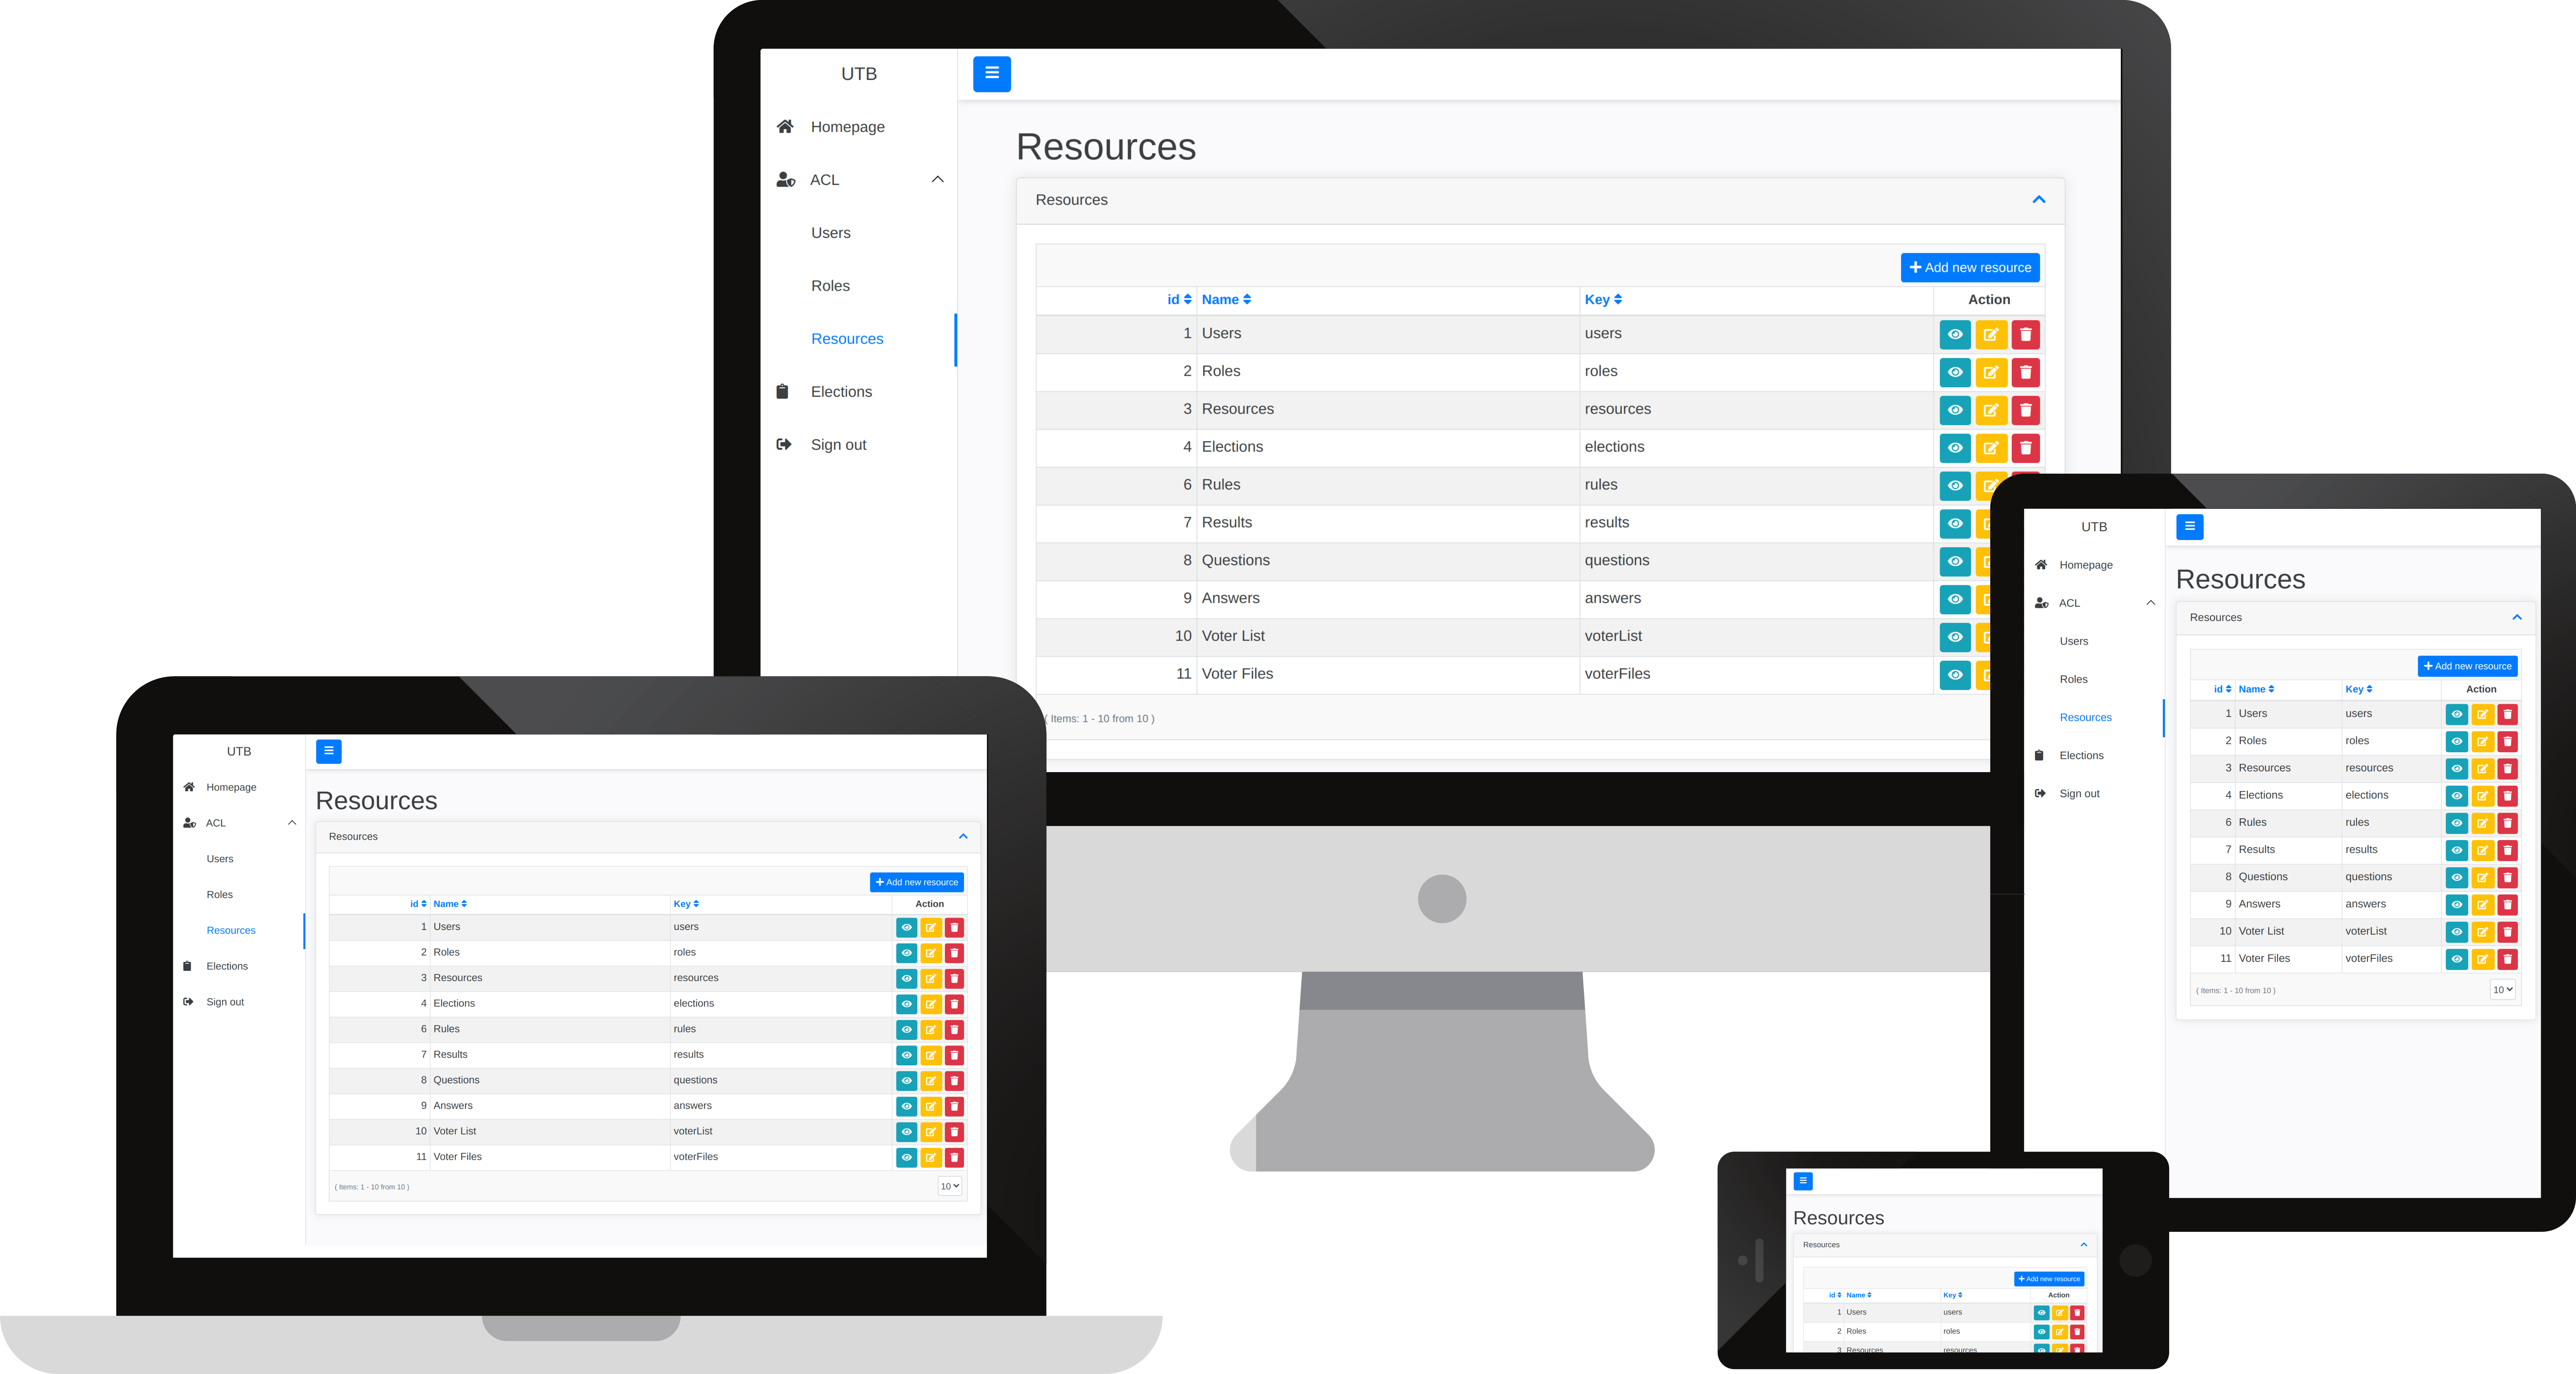
\includegraphics[width=\linewidth]{svg/mockup/datagrid.png}
	\captionsetup{width=\linewidth}
	\caption[Vzhled datagridu]{Vzhled datagridu (zdroj: vlastní, Freepik.com)}
	\label{mockup:login}
\end{figure}

Akce nad řádkem jsou typicky úlohy typu editace, mazání zobrazení detailu a~směřují na \textit{Signál} presenteru (metody \texttt{handle}). Jsou reprezentovány ikonami. Požadavek na~vymazání řádku (záznamu) je navíc opatřen potvrzovacím dialogovým oknem, aby nedošlo k nechtěnému smazání při nechtěném kliknutí.

Datagridy jsou vytvářeny pomocí třídy \phpinline{App\Backend\Utils\DataGrid\Datagrid}, která zefektivňuje způsob vytváření jednotlivých gridů díky zapouzdření často používaných konstrukcí. Tím se nejen výsledný kód v presenterech zjednoduší, ale zároveň gridy napříč aplikací mají stejné chování a na všechny se aplikuje stejná logika. Tímto přístupem se také podstatně usnadní změny ovlivňující všechny gridy - například změna ikony se projeví všude.

%\end{comment}

\n{1}{Zpracování hlasovacích lístků} \label{section:zpracovaniHlasu}
Nejcitlivější částí aplikace je bez pochyb právě práce s hlasovacími lístky, proto jí byla věnována samostatná část.
\n{2}{Odesílání hlasů}
\n{3}{Zpracování na straně klienta}

\n{3}{Zpracování na straně serveru}

\n{2}{Ukládání hlasů}

\n{2}{Počítání hlasů}

\n{2}{Výsledky}



% ============================================================================ %
\nn{Závěr}
Text závěru.

% ============================================================================ %

 % Hlavni text prace

\OdsazovaniOdstavcuStop

% ============================================================================ %
%\seznamlitbib


\tolerance=100
\emergencystretch=1em
\hyphenpenalty=10
\hbadness=10000
\clearpage
	\phantomsection
	\addcontentsline{toc}{section}{Seznam použité literatury}

	\begin{thebibliography}{99}
	
\bibitem{GoldsmithCaseSR}
GOLDSMITH, Ben a Holly RUTHRAUFF. \textit{Case Study Report on Electronic Voting in the Netherlands}. [b.r.]
Dostupné také~z:~https://www.ndi.org/sites/default/files/5{\_}Netherlands.pdf

\bibitem{Valasek2020}
VALÁŠEK, Michal. Lesk a bída elektronických voleb. \textit{Altair.blog} [online]. Praha: Valášek, 2020 [cit. 2021-5-12]. Dostupné~z:~https://www.altair.blog/2020/07/evolby

\bibitem{estoniaTurnout}
ALVAREZ, R. Michael, Thad E. HALL a Alexander H. TRECHSEL. Internet Voting in Comparative Perspective: The Case of Estonia. \textit{PS: Political Science \& Politics}. Cambridge University Press, 2009, \textbf{42}(3), 497-505. Dostupné~z:~doi:10.1017/S1049096509090787

\bibitem{swissTurnout}
GERMANN, Micha a Uwe SERDÜLT. Internet voting and turnout: Evidence from Switzerland. \textit{Electoral Studies}. 2017, \textbf{47}, 1-12. ISSN 0261-3794. Dostupné~z:~doi:10.1016/j.electstud.2017.03.001

\bibitem{Schneier1996}
SCHNEIER, Bruce. \textit{Applied cryptography: protocols, algorithms, and source code in C}. 2nd edition. Indianapolis: Wiley, 1996. ISBN 978-0471117094.

\bibitem{4285237}
ANANE, Rachid, Richard FREELAND a Georgios THEODOROPOULOS. E-Voting Requirements and Implementation. In: \textit{The 9th IEEE International Conference on E-Commerce Technology and The 4th IEEE International Conference on Enterprise Computing, E-Commerce and E-Services (CEC-EEE 2007)}. 2007, s.~382-392. Dostupné~z:~doi:10.1109/CEC-EEE.2007.42

\bibitem{QADAH2007376}
QADAH, Ghassan Z. a Rani TAHA. Electronic voting systems: Requirements, design, and implementation. \textit{Computer Standards \& Interfaces}. 2007, \textbf{29}(3), 376-386. ISSN 0920-5489. Dostupné~z:~doi:10.1016/j.csi.2006.06.001

\bibitem{10.1007/978-3-642-03315-5_13}
NOVOTNÝ, Marián. Design and Analysis of a Practical E-Voting Protocol. In: \textit{The Future of Identity in the Information Society}. Berlin: Springer, 2009, s.~170-183. ISBN 978-3-642-03315-5. Dostupné~z: doi:10.1007/978-3-642-03315-5\_13

\bibitem{receiptFree}
BARROS, Charles a Diego PIMENTA. A Receipt-Freei-Voting System Based on Blind Signatures and Anonymous IDs. In: \textit{Simpósio Brasileiro em Segurança da Informação e de Sistemas Computacionais (SBSEG)}. Brazílie, 2018. Dostupné~také~z: https://sol.sbc.org.br/index.php/sbseg/article/download/4277/4208/

\bibitem{eduId}
Shibboleth SP 3. \textit{EduID.cz} [online]. Praha: CESNET, z. s. p. o., 1996, 2020-03-26 11:56 [cit. 2020-11-23]. Dostupné~z: https://www.eduid.cz/cs/tech/sp/shibboleth

\bibitem{volebniRadUTB}
UNIVERZITA TOMÁŠE BATI VE ZLÍNĚ. \textit{Volební řád akademického senátu Univerzity Tomáše Bati ve Zlíně}. Zlín, 2016. Dostupné~také~z: https://www.utb.cz/univerzita/uredni-deska/vnitrni-normy-a-predpisy/vnitrni-predpisy/

\bibitem{volebniRadFAI}
UNIVERZITA TOMÁŠE BATI VE ZLÍNĚ. \textit{Volební řád Akademického senátu Fakulty aplikované informatiky Univerzity Tomáše Bati ve Zlíně}. Zlín, 2017. Dostupné~také~z: https://fai.utb.cz/o-fakulte/uredni-deska/vnitrni-normy-fai/vnitrni-predpisy-fai/

\bibitem{chaum}
CHAUM, David. Blind Signatures for Untraceable Payments. In: \textit{Advances in Cryptology}. Boston: Springer, 1983, s.~199-203. ISBN 978-1-4757-0602-4. Dostupné~také~z: https://sceweb.sce.uhcl.edu/yang/teaching/csci5234WebSecurityFall2011/Chaum-blind-signatures.PDF

\bibitem{Vejvoda2015}
VEJVODA, Bc. Petr. \textit{Elektronický volební systém}. Liberec, 2015. Diplomová práce. Technická univerzita v Liberci. Vedoucí práce Prof. Ing. Zdeněk Plíva, Ph.D.

\bibitem{Silhavy2009}
ŠILHAVÝ, Ing. Radek. \textit{Experimentální ověření distribuovaného volebního schématu}. Zlín, 2009. Disertační práce. Univerzita Tomáše Bati ve Zlíně. Vedoucí práce Doc. Ing. Zdenka Prokopová, CSc.

\bibitem{Kucharczyk}
KUCHARCZYK, Marcin. Blind Signatures in Electronic Voting Systems. In: \textit{Computer Networks}. Berlin: Springer, 2010, s.~349-358. ISBN 978-3-642-13861-4.

\bibitem{rsa}
RIVEST, Ronald, Adi SHAMIR a Leonard ADLEMAN. A method for obtaining digital signatures and public-key cryptosystems. \textit{Communications of the ACM}. New York: ACM, 1978, \textbf{21}(2), 120-126. Dostupné~také~z: https://people.csail.mit.edu/rivest/Rsapaper.pdf

\bibitem{RsaAdventures}
YUN, Cathie. Adventures with RSA Blind Signing. \textit{Medium.com} [online]. USA: Medium.com, 2021 [cit. 2021-5-11]. Dostupné~z: https://cathieyun.medium.com/adventures-with-rsa-blind-signing-397035585121

\bibitem{Haska2016}
HAŠKA, David. \textit{Porovnání PHP frameworků pro tvorbu internetové aplikace}. Praha, 2016. Bakalářská práce. Vysoká škola ekonomická v Praze. Vedoucí práce Filip Vencovský.

\bibitem{FowlerMVC}
FOWLER, Martin. \textit{Patterns of enterprise application architecture}. Boston: Addison-Wesley, 2003. Addison-Wesley signature series. ISBN 978-0321127426.

\bibitem{Vrana2013}
VRÁNA, J. \textit{1001 tipů a triků pro PHP}. Albatros Media a.s, 2013. ISBN 9788025139387.

\bibitem{zdrojakMVC}
BOREK, Bernard. Prezentační vzory z rodiny MVC. \textit{Zdroják.cz} [online]. Praha: Devel.cz Lab, 2009 [cit. 2021-5-7]. Dostupné~z: https://zdrojak.cz/clanky/prezentacni-vzory-zrodiny-mvc/

\bibitem{FowlerPassiveView}
FOWLER, Martin. Passive View. \textit{Martin Fowler} [online]. Chicago: Martin Fowler, 2006, 18. 7. 2006 [cit. 2021-5-9]. Dostupné~z: https://www.martinfowler.com/eaaDev/PassiveScreen.html

\bibitem{MVCmodel}
How should a model be structured in MVC? \textit{StackOverflow} [online]. 2018, [cit. 2021-5-9]. Dostupné~z: https://stackoverflow.com/a/5864000

\bibitem{NetteDocs}
\textit{Nette Docs: Dokumentace Nette 3.1} [online]. Praha: Nette Foundation, 2008 [cit. 2020-4-20]. Dostupné~z: https://doc.nette.org/cs/3.1/

\bibitem{NettePresentery}
Presentery. \textit{Nette 3.1 Docs} [online]. Praha: Nette Foundation, 2021 [cit. 2021-5-9]. Dostupné~z: https://doc.nette.org/cs/3.1/presenters\#toc-action-action

\bibitem{XssPrevention}
Cross Site Scripting Prevention Cheat Sheet \textit{OWASP} [online]. USA: OWASP, 2021 [cit. 2021-5-9]. Dostupné~z: https://cheatsheetseries.owasp.org/cheatsheets/\\Cross{\_}Site{\_}Scripting{\_}Prevention{\_}Cheat{\_}Sheet.html

\bibitem{Latte}
\textit{Latte - nejbezpečnější {\&} opravdu intuitivní šablony pro PHP} [online]. Praha: Nette Foundation, 2008 [cit. 2020-4-20]. Dostupné~z: https://latte.nette.org/cs/

\bibitem{NetteRoutovani}
Routování. \textit{Nette 3.1 Docs} [online]. Praha: Nette Foundation, 2021 [cit. 2021-5-9]. Dostupné~z: https://doc.nette.org/cs/3.1/routing

\bibitem{EvansDDD}
EVANS, Eric. \textit{Domain-driven Design: Tackling Complexity in the Heart of Software}. Boston: Addison-Wesley, 2004. ISBN 0-321-12521-5.

\bibitem{Boehmer2015}
BÖHMER, M. \textit{Návrhové vzory v PHP}. Albatros Media a.s, 2015. ISBN 9788025144756.

\bibitem{Martin2002}
MARTIN, Robert C. \textit{Agile Software Development, Principles, Patterns, and Practices}. New York: Pearson, 2002. ISBN 978-0135974445.

\bibitem{NetteRefactoring}
GRUDL, David. Nette Framework: Refactoring. \textit{Zdroják.cz} [online]. Praha: Devel.cz Lab, 2009 [cit. 2021-5-9]. Dostupné~z: https://zdrojak.cz/clanky/nette-framework-refactoring/

\bibitem{Planette}
Best practice: formuláře jako komponenty. \textit{Nette} [online]. Praha: Nette Foundation, 2021 [cit. 2021-5-7]. Dostupné~z: https://pla.nette.org/cs/best-practice-formulare-jako-komponenty\#toc-ui-control

\bibitem{Tracy}
\textit{Tracy: ladicí nástroj se kterým je radost chybovat} [online]. Praha: Nette Foundation, 2021 [cit. 2021-5-7]. Dostupné~z: https://tracy.nette.org/

\bibitem{Bootstrap}
\textit{Bootstrap v4.6} [online]. USA: Bootstrap, 2021 [cit. 2021-5-12]. Dostupné~z: https://getbootstrap.com/docs/4.6/

\bibitem{FontAwesome}
\textit{FontAwesome} [online]. USA: Fonticons, 2021 [cit. 2021-5-12]. Dostupné~z: https://getbootstrap.com/docs/4.6/

\bibitem{ContributteDataGrid}
\textit{Contributte Datagrid: DataGrid for Nette framework} [online]. Praha: Contributte, 2021 [cit. 2021-5-8]. Dostupné~z: https://contributte.org/packages/contributte/datagrid/

\bibitem{NetteForms}
Validace formulářů. \textit{Nette 3.1 Docs} [online]. Praha: Nette Foundation, 2021 [cit. 2021-5-9]. Dostupné~z: https://doc.nette.org/cs/3.1/form-validation

\bibitem{Sklar2018}
SKLAR, D. a J. POKORNÝ. \textit{PHP 7: praktický průvodce nejrozšířenějším skriptovacím jazykem pro web: Encyklopedie Zoner Press}. Zoner Press, 2018. ISBN 9788074133633.

\bibitem{Validace1}
TRUTH, Serge. Do Not Rely On Client-Side Validation. \textit{Security Innovation} [online]. USA: Security Innovation, 2011 [cit. 2021-5-9]. Dostupné~z: https://blog.securityinnovation.com/blog/2011/07/do-not-rely-on-client-side-validation.html

\bibitem{Validace2}
Is HTML5 input pattern validation sufficient (or even relevant) for client-side validation? \textit{Information Security Stack Exchange} [online]. USA: Stack Exchange, 2017 [cit. 2021-5-9]. Dostupné~z: https://security.stackexchange.com/questions/169771/is-html5-input-pattern-validation-sufficient-or-even-relevant-for-client-side

\bibitem{Validace3}
JOVANOVIC, Janko. Web Form Validation: Best Practices and Tutorials. \textit{Smashing Magazine} [online]. USA: Smashing Magazine, 2009 [cit. 2021-5-9]. Dostupné~z: https://blog.securityinnovation.com/blog/2011/07/do-not-rely-on-client-side-validation.html

\bibitem{phpseclibBlinding}
WIGGINTON, Jim. Crypt\_RSA. \textit{Phpseclib API Documentation} [online]. USA: Jim Wigginton [cit. 2021-5-10]. Dostupné~z: https://api.phpseclib.com/1.0/Crypt\_RSA.html


	\end{thebibliography}

\tolerance=1
\emergencystretch=\maxdimen
\hyphenpenalty=10000
\hbadness=10000

% ============================================================================ %
% ============================================================================ %
% Encoding: UTF-8 (žluťoučký kůň úpěl ďábelšké ódy)
% ============================================================================ %

\seznamzkr

\begin{tabular}{ll}
2FA 		& Two-Factor Authentication \\
AES 		& Advanced Encryption Standard \\
AES-GCM 	& AES Galois/Counter Mode \\
ACL 		& Access Control List \\
AJAX 	& Asynchronous JavaScript and XML \\
CSRF 	& Cross-Site Request Forgery \\
CSS		& Cascading Style Sheets \\
DDD 		& Domain Driven Design \\
GDPR		& General Data Protection Regulation \\
GNU GPL	& GNU General Public License \\
HTTP 	& Hyper Text Transfer Protocol \\
JS		& JavaScript \\
JSON		& JavaScript Object Notation \\
LDAP		& Lightweight Directory Access Protocol \\
MVC 		& Model View Controller \\
MVP 		& Model View Presenter \\
RSA		& Rivest–Shamir–Adleman \\
RSA-OAEP	& RSA Optimal Asymmetric Encryption Padding \\
SRP 		& Single Responsibility Principle \\
SQL		& Structured Query Language \\
VPS		& Virtual Private Server \\
WYSIWYG 	& What You See Is What You Get \\
XML 		& Extensible Markup Language \\
XSS 		& Cross-site Scripting \\
\end{tabular}

% ============================================================================ % % Seznam zkratek


% ============================================================================ %
\seznamobr  % Seznam je generován automaticky


% ============================================================================ %
\seznamtab  % Seznam je generován automaticky


\seznamkodu

% ============================================================================ %
% ============================================================================ %
% Encoding: UTF-8 (žluťoučký kůň úpěl ďábelšké ódy)
% ============================================================================ %

\listofappendices

\priloha{Adresářová struktura aplikace}
\label{priloha:adresare}
\dirtree{%
 .1 /.
 .2 app.
 .3 Backend.
 .4 Classes.
 .4 Presenters.
 .5 templates.
 .4 Utils.
 .3 config.
 .3 Core.
 .4 Classes.
 .4 Presenters.
 .5 templates.
 .4 Utils.
 .3 Forms.
 .3 Frontend.
 .4 Classes.
 .4 Presenters.
 .5 templates.
 .3 Models.
 .4 Entities.
 .4 Factories.
 .4 Mappers.
 .5 Db.
 .4 Traits.
 .3 Repositories.
 .3 Router.
 .3 Bootstrap.php.
 .2 bin.
 .2 keys.
 .2 log.
 .2 temp.
 .2 vendor.
 .2 www.
 .2 www\_backend.
 .2 composer.json.
}

\priloha{Založení a správa voleb v aplikaci}
\subsection*{Založení}
\begin{itemize}
	\item Kliknutím na tlačítko vytvoření nových voleb (v záhlaví datagridu) je zobrazen formulář pro editaci voleb (Obrázek PII.1).
	\begin{figure}[h]
	\centering
	\includegraphics[width=\linewidth]{tex/attachements/noveVolbyForm.png}
	\captionsetup{width=\linewidth}
	\caption*{Obrázek P II.1 Formulář založení nových voleb (zdroj: vlastní)}
\end{figure}
	\item Po vyplnění a odeslání formuláře lze uložené hodnoty upravit pomocí editačního tlačítka na příslušném řádku v datagridu (Obrázek PII.2).
	\item Na detail voleb lze přejít kliknutím na tlačítko detailu v příslušném řádku datagridu.
	\begin{figure}[h]
	\centering
	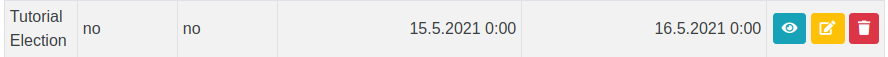
\includegraphics[width=\linewidth]{tex/attachements/noveVolbyGrid.png}
	\captionsetup{width=\linewidth}
	\caption*{Obrázek P II.2 Řádek datagridu (zdroj: vlastní)}
\end{figure}
\end{itemize}






\subsection*{Otázky}
Nastavení otázek se provádí na záložce \textit{Questions}. Již přidané otázky jsou zobrazeny v~datagridu a lze je upravovat. Nové otázky se přidávají tlačítkem v záhlaví datagridu. Název otázky slouží pro orientaci v seznamu definovaných otázek, voliči není zobrazen. Každá otázka musí mít nastaven minimální a maximální možný počet odpovědí. Limit se při validaci aplikuje pouze pokud je vybrána alespoň jedna odpověď. Pro nepovinné otázky tedy není nutné zadávat limit 0 (aplikace to ani nepovolí). Dalšími poli jsou text samotné otázky a nastavení zda je odpověď na otázku vyžadována. 

Toto umožňuje dvojí řešení, pokud je vyžadována možnost zdržet se volby (hlasování). Nepovinná otázka umožňuje neodpovídat, ale ve výsledcích voleb není zohledněno, že volič se rozhodl neodpovědět (jinak než porovnáním počtu ostatních možností a~odevzdaných hlasů). Druhým řešením je volbu ,,Zdržel se'' zavést jako jednu z možných odpovědí. V takovém případě bude zohleděna tato volba i ve výsledcích. Obdobně by se dalo dívat i na odpověďi ,,Nechci odpovídat'', ,,Nevím'' apod.

V poslední části formuláře je možné přidávat jednotlivé odpovědi. 
\begin{itemize}
\item Další odpovědi lze přidávat kliknutím na tlačítko plus, odebírat tlačítkem minus. 
\item Minimum a maximum možných definic odpovědí je definováno ve zdrojovém kódu formuláře. Výchozí hodnoty jsou minimálně jedna a maximálně padesát odpovědí. 
\item Výchozí hodnoty lze přepsat metodami: 
\begin{itemize}
 \item \phpinline{QuestionForm::setMultiplierCopies($copies)} pro minimum a
 \item \phpinline{QuestionForm::setMultiplierMaxCopies($maxCopies)} pro maximum.
\end{itemize}
Tyto metody je ideální volat v místě vytváření formuláře, tedy v~\phpinline{ElectionPresenter::createComponentQuestionForm()}. 
\item Změnit výchozí hodnoty napřímo v kódu lze ve třídě \texttt{HasMultiplier}\footnote{\Verb{App\Forms\HasMultiplier}}.

\end{itemize}

Po odeslání formuláře jsou data uložena a otázky i odpovědi je možné upravit opět pomocí editačního tlačítka. Celou otázku lze smazat červeným tlačítkem odpoadkového koše. Jednotlivé odpovědi lze mazat ze samostatné záložky \textit{Answers}.

\subsection*{Seznam voličů}
Seznam voličů vzniká z CSV souboru nahraného prostřednictvím aplikace. 
\begin{itemize}
	\item Aktuální seznam voličů je dostupný přes záložku \textit{Voter List}.
	\item Na záložce \textit{Voter Files} je seznam již nahraných souborů.
	\item Nové soubory lze nahrát prostřednictvím kontextového menu dostupného po~kliknutí na ikonu ozubeného kola.
	\item Kterýkoli z nahraných souborů lze aplikovat pro dané volby kliknutím na zelené tlačítko ,,Apply''.
	\item Nahrané soubory lze také smazat nebo stáhnout do počítače a zobrazit jejich obsah.
	\item Smazání nahraného souboru neovlivní již aplikovaný seznam voličů.
\end{itemize}

\subsection*{Spuštění voleb}
Před aktivací voleb je nutné nahrát veřejnou část RSA klíče volební komise prostřednictvím kontextového menu (ozubené kolo). Tento klíč by měl být uložen na~bezpečném místě a volební komise by měla zajistit jeho patřičnou zálohu v případě ztráty nebo poškození originálu. Není možné použít klíč chráněný heslem (použitá knihovna \texttt{phpseclib} použití takového klíče nicméně umožňuje a aplikace by k tomu mohla být upravena). Úspěšně nahraný klíč je viditelný na záložce \textit{Overview} v~tabulce s šifrovacími klíči.

V tuto chvíli je možné volby aktivovat opět prostřednictvím ozubeného kola.

\subsection*{Ukončení voleb}

\begin{itemize}
	\item Po skončení období nastaveného pro dané volby jsou zpřístupněny další akce na~detailu voleb.
	\item Přes kontextové menu je nyní možné nahrát privátní část klíče volební komise.
	\item Po úspěšném nahrání klíče je tento také vidět na záložce \textit{Overview}
	\item Kliknutím na tlačítko ,,Decrypt and count ballots'' na záložce \textit{Results} jsou spočítány odevzdané hlasy
	\item Výsledky voleb jsou zobrazovány i voličům
	\item Pomocí kontextového menu je možné stáhnout volební protokol
	\item Volby je možné deaktivovat přes kontextové menu, neaktivní volby se již nezobrazují voličům.
	\item Ukončené volby včetně všech podstatných náležitostí je možné smazat červeným tlačítkem odpadkového koše v datagridu všech voleb. Veškeré záznamy spojené s~těmito volbami budou rovněž odstraněny. Tato akce je nevratná!
\end{itemize}




\priloha{Průběh voleb z pohledu voliče}
\begin{figure}[h]
	\centering
	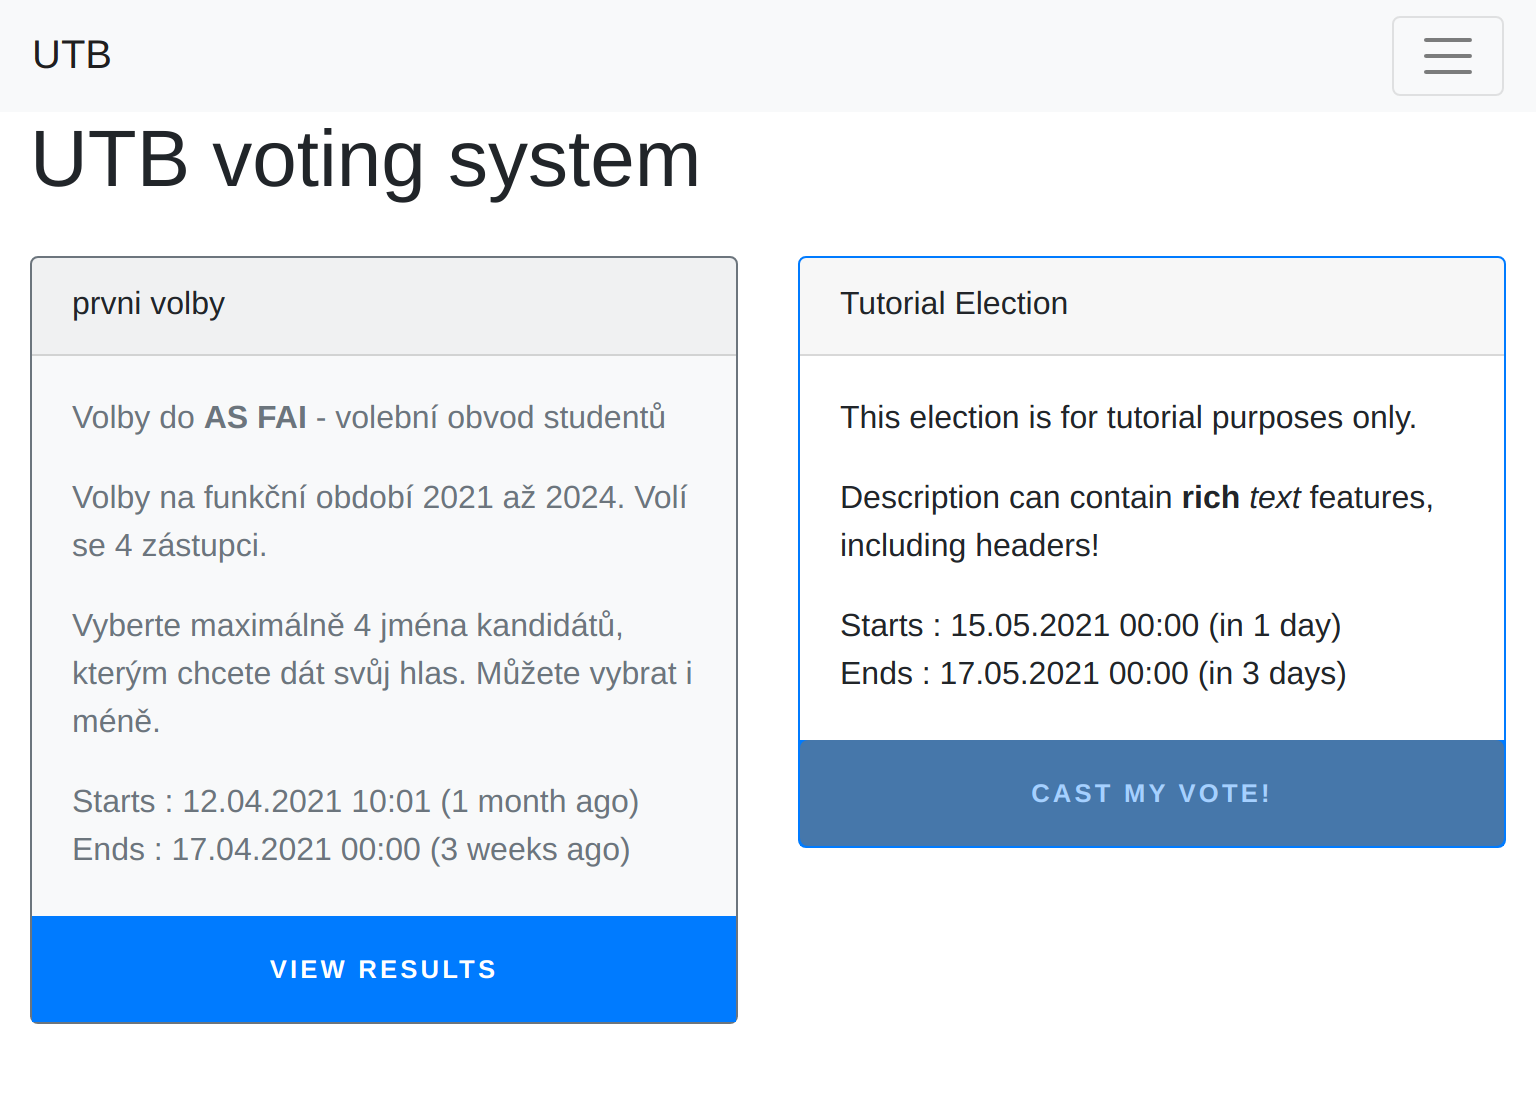
\includegraphics[width=\linewidth]{graphics/attachements/volbyPrehledDouble.png}
	\captionsetup{width=\linewidth}
	\caption*{Popisek obrázku (zdroj: vlastní)}
\end{figure}

\begin{figure}[h]
	\centering
	\includegraphics[width=\linewidth]{graphics/attachements/volbyCompared.png}
	\captionsetup{width=\linewidth}
	\caption*{Popisek obrázku (zdroj: vlastní)}
\end{figure}

\begin{figure}[h]
	\centering
	\includegraphics[width=\linewidth]{graphics/attachements/volbyCompared2.png}
	\captionsetup{width=\linewidth}
	\caption*{Popisek obrázku (zdroj: vlastní)}
\end{figure}

\begin{figure}[h]
	\centering
	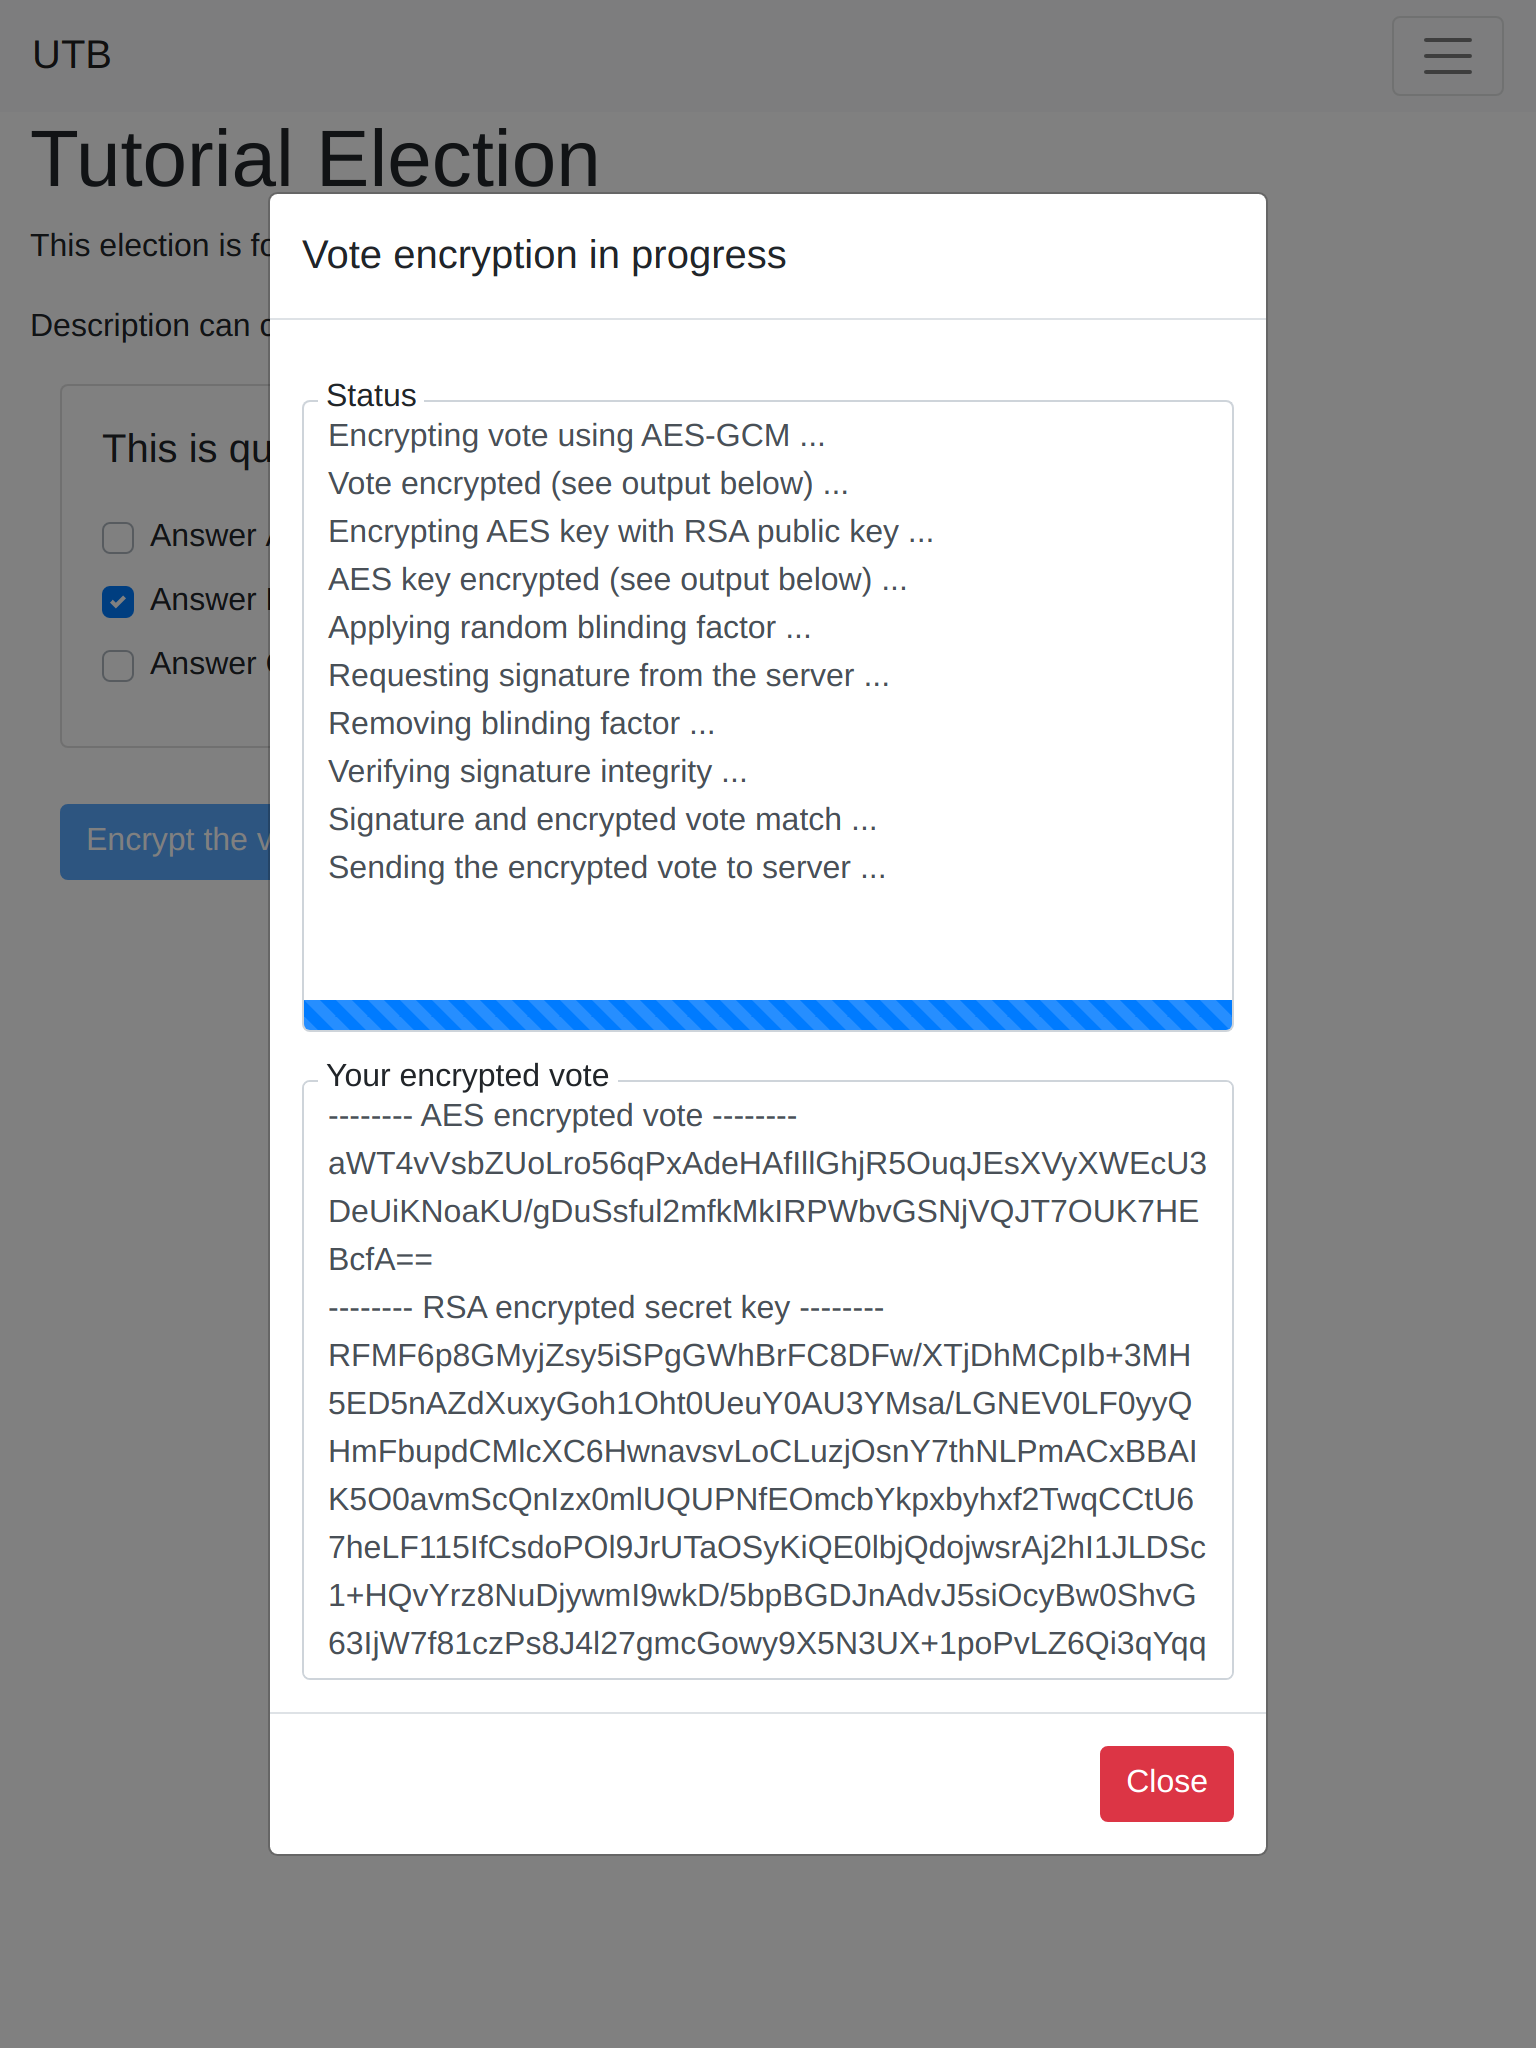
\includegraphics[width=\linewidth]{graphics/attachements/volbyDetails.png}
	\captionsetup{width=\linewidth}
	\caption*{Popisek obrázku (zdroj: vlastní)}
\end{figure}

\priloha{Balíčky třetích stran}
\subsection*{Datagrid}

% ============================================================================ %
 % Prilohy


% ============================================================================ %

\end{document}

% ============================================================================ %
